\documentclass[12pt,a4paper]{report}
\usepackage[english]{babel}
\usepackage{newlfont}
\usepackage{ amssymb }
\usepackage{algorithm}
\usepackage{algpseudocode}
\usepackage{graphicx}
\usepackage{ wasysym }
\usepackage{ upgreek }
\usepackage{verbatim}
\usepackage{amsmath}

\usepackage[T1]{fontenc}
\usepackage{beramono}
\usepackage{listings}
\usepackage{xcolor}

\usepackage{subfig}
               
\definecolor{dkgreen}{rgb}{0,0.6,0}
\definecolor{gray}{rgb}{0.5,0.5,0.5}
\definecolor{mauve}{rgb}{0.58,0,0.82}

\lstdefinestyle{myScalastyle}{
  frame=tb,
  language=scala,
  aboveskip=3mm,
  belowskip=3mm,
  showstringspaces=false,
  columns=flexible,
  basicstyle={\small\ttfamily},
  numbers=none,
  numberstyle=\tiny\color{gray},
  keywordstyle=\color{blue},
  commentstyle=\color{dkgreen},
  stringstyle=\color{mauve},
  frame=single,
  breaklines=true,
  breakatwhitespace=true,
  tabsize=3,
}

% MATHEMATICAL SYMBOLS ENCODIN
\newcommand\domain{D}
\newcommand\systemModel{\mathcal{Z}}
\newcommand\systemName{GFDM}
\newcommand\globalQuery{\varphi}
\newcommand\algebraQuery{\varphi_{RA}}
\newcommand\sqlQuery{\varphi_{sql}}
\newcommand\rollUpQuery{\varphi_{rollUp}}
\newcommand\expandedQuery{\varphi_{E}}
\newcommand\targetGraph{\mathcal{G}}
\newcommand\sourceGraph{\mathcal{S}}
\newcommand\integrationGraph{\mathcal{I}}
\newcommand\targetGraphVertex{V_{\targetGraph}}
\newcommand\targetGraphEdge{E_{\targetGraph}}
\newcommand\targetMultidimensionalGraphVertex{V_{\multidimensionalGraph}}
\newcommand\targetMultidimensionalGraphEdge{E_{\multidimensionalGraph}}
\newcommand\integrationGraphVertex{V_{\integrationGraph}}
\newcommand\integrationGraphEdge{E_{\integrationGraph}}
\newcommand\sourceGraphVertex{V_{\sourceGraph}}
\newcommand\sourceGraphEdge{E_{\sourceGraph}}

\newcommand\implicitRollUp{}
\newcommand\subject{S}
\newcommand\predicate{P}
\newcommand\object{O}

\newcommand\concept{C}
\newcommand\feature{F}
\newcommand\idFeature{\feature^{id}}
\newcommand\wrapper{W}
\newcommand\lut{W_{lut}}
\newcommand\attribute{A}
\newcommand\hasFeature{hasFeature}
\newcommand\hasAttribute{hasAttribute}
\newcommand\sameAs{sameAs}

\newcommand\view{\mathcal{V}}

\newcommand\triple[1]{#1_{\set{\subject,\predicate,\object}}}
\newcommand\multidimensionalCube{\mathcal{MC}}

\newcommand\factCube{\mathcal{F}_{\multidimensionalCube}}
\newcommand\dimensionCube{\mathcal{D}_{\multidimensionalCube}}
\newcommand\levelCube{\mathcal{L}_{\multidimensionalCube}}
\newcommand\measureCube{\mathcal{M}_{\multidimensionalCube}}

\newcommand\fact{\mathcal{F}}
\newcommand\dimension{\mathcal{D}}
\newcommand\level{\mathcal{L}}
\newcommand\measure{\mathcal{M}}
\newcommand\levelsFunLabel{levels}
\newcommand\dimensions{dimensions}
\newcommand\levelsFundefinition{\levelsFunLabel:\dimension\rightarrow \langle \level \rangle}
\newcommand\dimensionsFundefinition{\dimensions:\fact\rightarrow \langle \dimension \rangle}
\newcommand\dimensionsDefinition{\dimensions:\fact\rightarrow \langle \dimension \rangle}
\newcommand\multidimensionalGraph{\mathcal{MG}}
\newcommand\aggregatingFunction{\mathcal{AF}}
\newcommand\aggregatingFunctionFunLabel{aggregates}
\newcommand\aggregatingFunctionDefinition{\aggregatingFunctionFunLabel: \aggregatingFunction \rightarrow \langle \measure \rangle}
\newcommand\partOfFunLabel{partOf}
\newcommand\partOfFunDefinition{\partOfFunLabel:\level \rightarrow \level'}
\newcommand\measuresFunLabel{measures}
\newcommand\measuresFunDefinition{\measuresFunLabel:\fact \rightarrow \set{\measure}}
\newcommand\mapping{mapping}
\newcommand\functionsFunLabel{functions}
\newcommand\functionsFunDefinition{\functionsFunLabel:\fact\rightarrow \aggregatingFunction}

\newcommand\id{id}
\newcommand\levels{levels}
\newcommand\measures{measures}
\newcommand\features{features}
\newcommand\levelsWithIdFeature{levelsWithIdFeature}
\newcommand\levelsIdFeature{levelsIdFeature}
\newcommand\aggregatingFunctions{aggregatingFunctions}
\newcommand\lowerGranularityLevel{lowerGranularityLevel(\dimension)}
\newcommand\higherGranularityLevel{higherGranularityLevel(\dimension)}
\newcommand\set[1]{\langle #1 \rangle}

\newcommand\dimensionQuery{\globalQuery_{\dimension}}

% MATHEMATICAL SYMBOLS ENCODING

\algnewcommand\algorithmicforeach{\textbf{for each}}
\algdef{S}[FOR]{ForEach}[1]{\algorithmicforeach\ #1\ \algorithmicdo}

% ENUMERATION HIERARCHY
\renewcommand{\labelenumii}{\arabic{enumi}.\arabic{enumii}}
\renewcommand{\labelenumiii}{\arabic{enumi}.\arabic{enumii}.\arabic{enumiii}}
\renewcommand{\labelenumiv}{\arabic{enumi}.\arabic{enumii}.\arabic{enumiii}.\arabic{enumiv}}
% ENUMERATION HIERARCHY


\textwidth=450pt\oddsidemargin=0pt
\begin{document}
\begin{titlepage}
\begin{center}
{{\Large{\textsc{Alma Mater Studiorum $\cdot$ Universit\`a di
Bologna}}}} \rule[0.1cm]{15.8cm}{0.1mm}
\rule[0.5cm]{15.8cm}{0.6mm}
{\small{\bf SCUOLA DI SCIENZE\\
Corso di Laurea in Ingegneria e Scienze Informatiche }}
\end{center}
\vspace{15mm}
\begin{center}
{\LARGE{\bf Implicit Roll-Up over graph-based data integration system}}\\
\vspace{3mm}
%{\LARGE{\bf DELLA}}\\
%\vspace{3mm}
%{\LARGE{\bf TESI}}\\
\end{center}
\vspace{40mm}
\par
\noindent
\begin{minipage}[t]{0.47\textwidth}
{\large{\bf Relatore:\\
Matteo Golfarelli\\
\\
Collaboratori:\\
Oscar Romero, \\
Sergi Nadal 
}}
\end{minipage}
\hfill
\begin{minipage}[t]{0.47\textwidth}\raggedleft
{\large{\bf Presentata da:\\
Filippo Pistocchi}}
\end{minipage}
\vspace{20mm}
\begin{center}
{\large{\bf Sessione\\%inserire il numero della sessione in cui ci si laurea
Anno Accademico }}%inserire l'anno accademico a cui si è iscritti
\end{center}
\end{titlepage}

\tableofcontents
\listoffigures
\listofalgorithms

\chapter{Motivation} \label{Motivation}
The idea of this project came from the very well known necessity of facilitating as much as possible data scientist job of data wrangling, since to develop robust mathematical, machine learning and in particular deep models it is very important to have access to huge amount of (correct) data.
%
Nowadays, IoT and social networks are the main sources of big data, generating a massive amount of assets and stakeholders in companies will have to deal with heterogeneous dataset generated form different sources distributed all around the world.
%
Clearly handling such resources it is not a trivial task and to do so without specific tools it may be very complex.
%
Data integration systems have been developed to overcome these problems, with the purpose of re-conciliating huge amount of heterogeneous and distributed data sources, facilitating the process of knowledge discovering, making it possible to navigate data as a single integrated schema.
%
As we know from the literature there exists two main kind of architectures for data integration;
%
Physical data integration, is typically grounded in data warehouse and business intelligence systems and its biggest challenge is to structure and prepare data as multidimensional schema in order to analyse study fact as multidimensional models.
%
The aim of this technique is strictly analytical and the operation performed are aggregations over numerical data.
%
Typically this technique is mostly used to gather assets within a corporation, studying the business processes in order to define strategical decisions aimed to the internal improvement.
%
Virtual data integration aim, as opposite, is not grounded in just data aggregations.
%
Virtual data integration systems main goal is gathering huge amount of disconnected and heterogeneous data making easier the data wrangling process to data enthusiasts.

What we would like to do in this project is extend a virtual data integration system (graph-based) giving the possibility to support a multidimensional schema (with the shape of a graph) as data warehouses does.
%
This idea may lead to have both the advantages of virtual and physical data integration over a single system.

\section{Data integration techniques}
The aim of this section is to open a small parenthesis to describe the main data integration techniques, as we saw before virtual and physical data integration, detailing a bit more precisely their main characteristic in order to make it easier to understand the motivations behind this work.

\begin{itemize}
    \item Physical data integration
    \begin{itemize}
        \item Multidimensional model
        \item Multidimensional cube $\multidimensionalCube$
        \begin{itemize}
            \item Tell what $\fact$,$\dimension, \level, \measure$ are.
        \end{itemize}
        \item Roll-Up\footnote{https://en.wikipedia.org/wiki/Operation_Roll-Up} and Drill-Down
    \end{itemize}
    \item Virtual data integration
    \item Graph-based virtual data integration
    \begin{itemize}
        \item Ontology based data access
        \item Ontology mediated query
        \begin{itemize}
            \item LAV mappings.
            \item $\wrapper$
        \end{itemize}
    \end{itemize}
\end{itemize}

\section{Implicit Roll-Up philosophy}
From now on we will work on a graph virtual data integration, ontology mediated query based model, also KG (knowledge graph) based, that we will call $\systemModel$, in particular we will focus on a concerete implementation of $\systemModel$ called \systemName, more detail regarding this can be found in section \ref{Technology preliminaries}, but also in the real source TKDE publication \cite{TKDE}.
%
Let's define now the metadata describing a graph target schema target schema as $\targetGraph$ and a pattern matching or visual query over $\targetGraph$ as $\globalQuery$.
%
What we would like to do in this project is to develop a multidimensional graph schema that reuses the metadata structure of $\targetGraph$ and extend it giving the capability of supporting dimensions, levels and measures as multidimensional cubes $\multidimensionalCube$.
%
Let's identify this metadata structure as multidimensional graph, identified as $\multidimensionalGraph$.

The goal of the project then it will be trying to implement the multidimensional Roll-Up operation, one of the most important $\multidimensionalCube$ feature, over $\multidimensionalGraph$.
%
This may be very useful for different reasons;
%
%Let's define first the concept of fact $\fact$...
%
Considering that $\systemModel$ deals with lots of heterogeneous dataset, as declared in the introduction, it will be very likely to have data sources producing information, behaving to the same domain, but recorded in different granularity.
%
Therefore, the extension we would like to do in $\systemModel$ is, for each $\globalQuery$ over $\targetGraph$, or more specifically $\multidimensionalGraph$, trying to implicitly extrapolate a Roll-Up semantic and when it is possible to do so, deliver a result for $\globalQuery$ at the queried data granularity, considering the possibility of pushing up data behaving to the lowest data granularity to the queried data granularity available into $\multidimensionalGraph$, aggregating implicitly the numeric study measures.
%
Let's call this operation implicit Roll-Up.

The implicit Roll-Up then may be very useful for data scientists working over $\systemModel$ since it would come across to a subset of problems that data scientists face off daily.
%
As we can see Figure \ref{fig:Example} is showing a multidimensional graph $\multidimensionalGraph$ and a query $\globalQuery$ over $\multidimensionalGraph$ as a visual dashed red line.
%
The graph is describing a study fact related to \textit{Sales}, two study measures, respectively the \textit{total revenue} and the \textit{number of unit} and three dimensions (\textit{spatial}, \textit{temporal} and \textit{product}), each one having three granularity levels.
%
Let's focus now just on the \textit{spatial} dimension, that have \textit{City}, \textit{Region} and \textit{Country} as vertexes.
%
Given the semantic of $\globalQuery$, it is very intuitive that the user who triggered $\globalQuery$ is interested into the \textit{Region} granularity level for the \textit{spatial} dimension.
%
What we want our system to do is not just giving as result just the data at \textit{Region} granularity level, as \systemName\, would already do, but a total Roll-Up for the entire \textit{spatial} dimension, for all the lower granularity levels than the queried one, trying to deliver also data at \textit{City} granularity to \textit{Region} where possible, performing implicit aggregations over the queried measures granularity (this operation will clearly have to be done also for all the other queried dimensions).
%
\begin{figure} [ht]
    \fbox{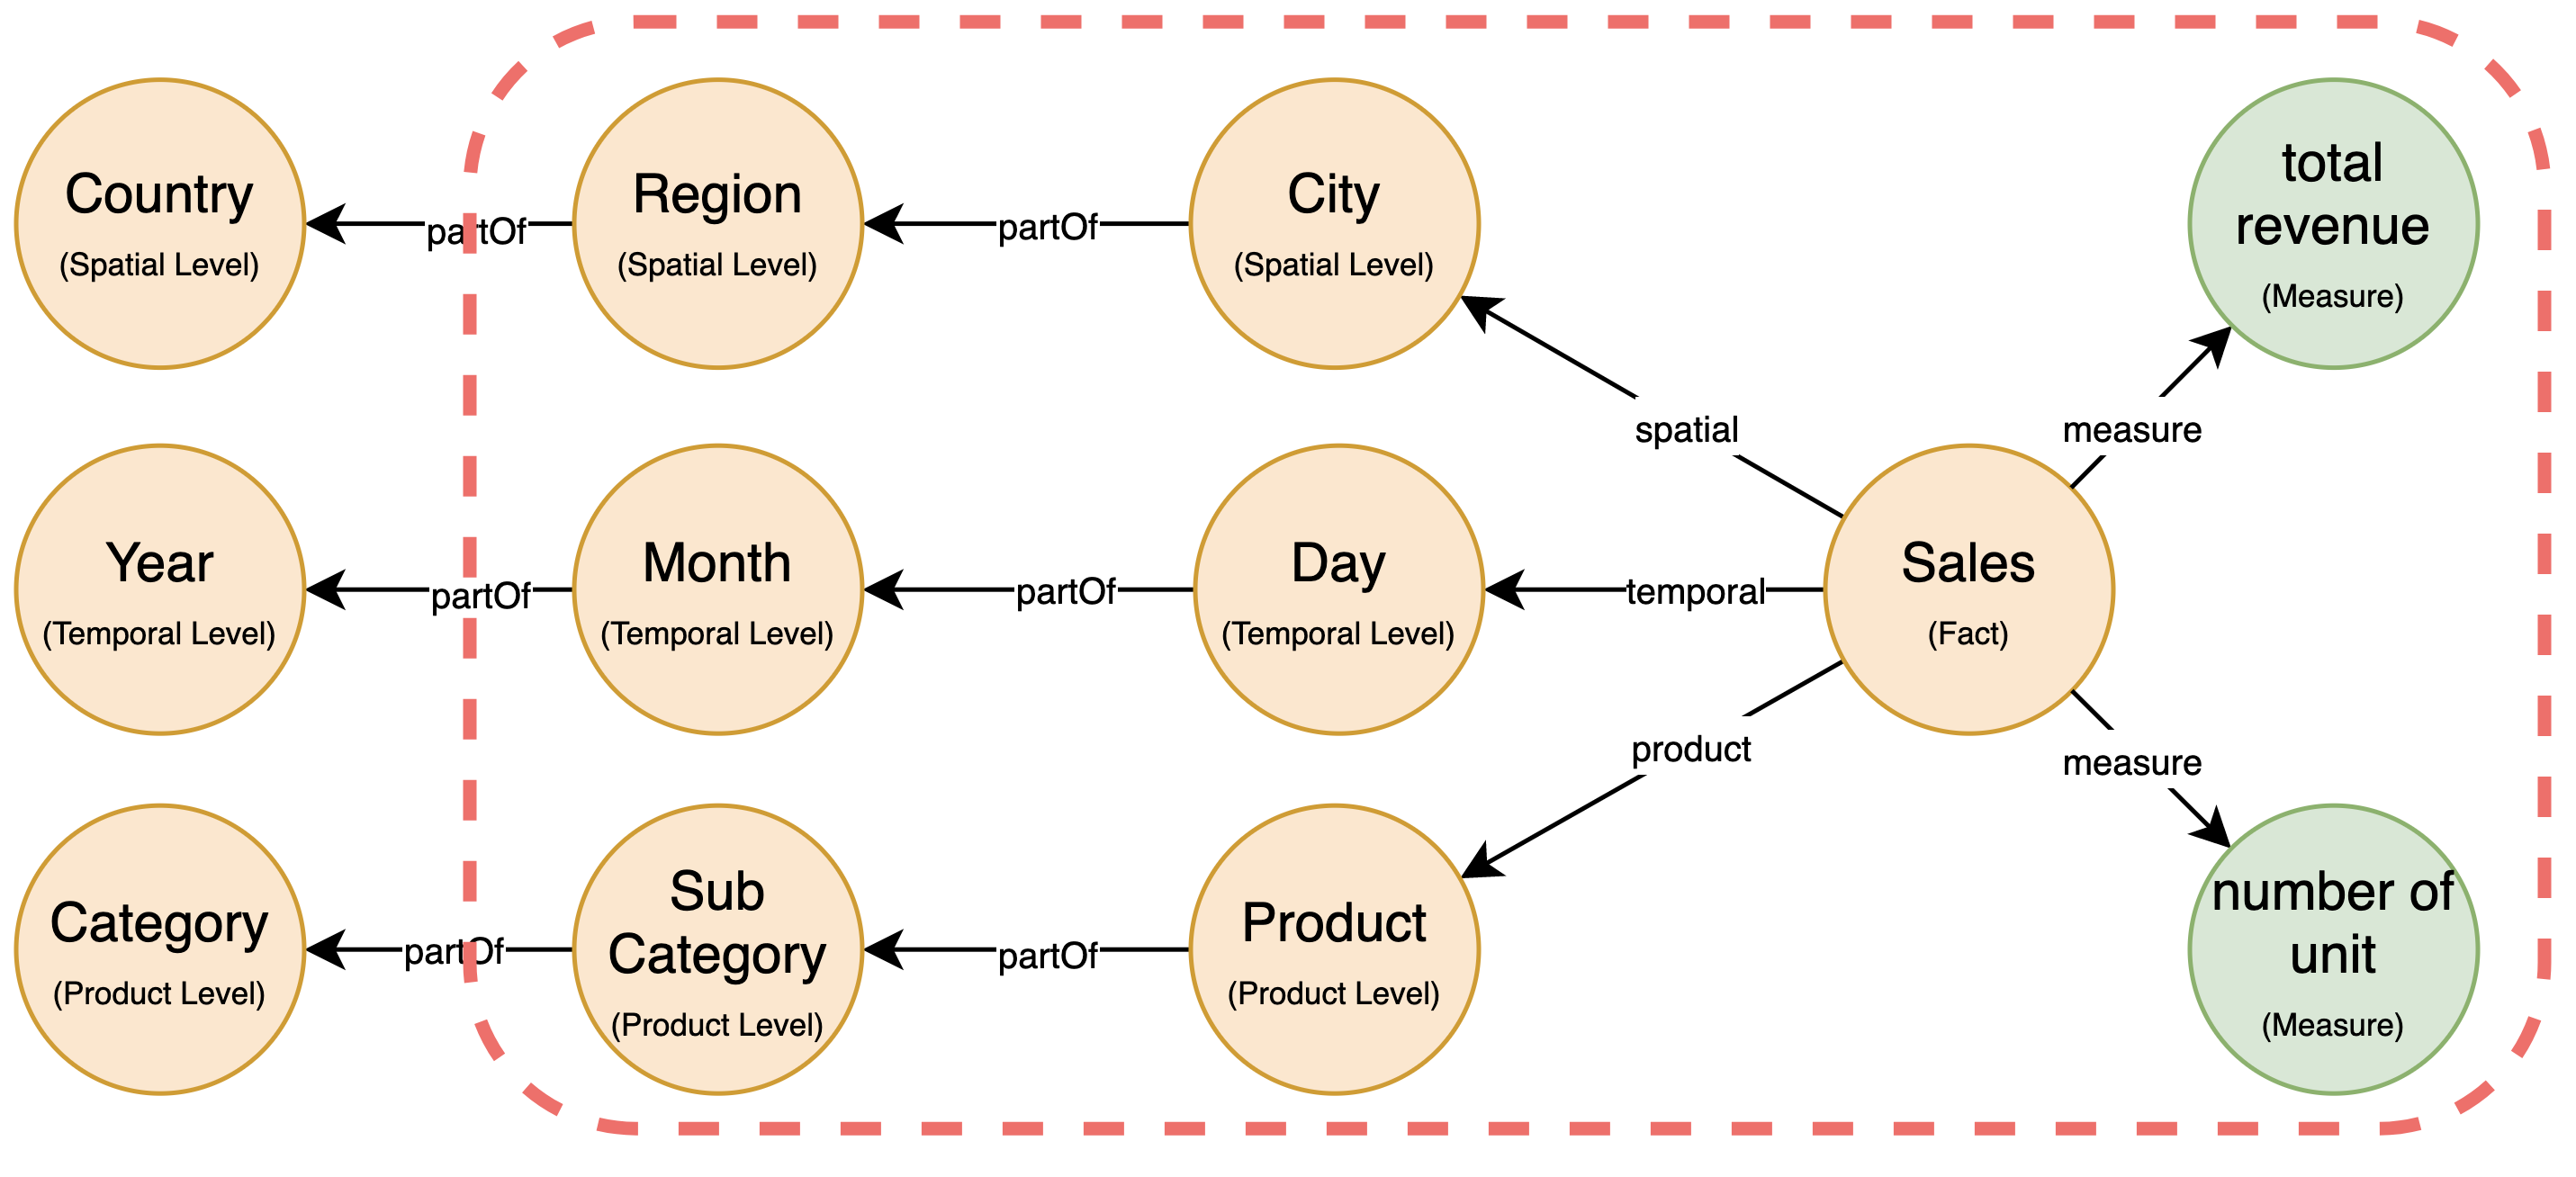
\includegraphics[width=\linewidth]{img/example.png}}
    \caption{Idea of a simplified multidimensional graph $\multidimensionalGraph$ having three different granularity level for three dimension and two numerical data. Also a query $\globalQuery$ have been depicted as a dashed red line.}
    \label{fig:Example}
\end{figure}

The advantages of an implicit Roll-Up operation in this case would be twofold;
%
Firstly this operation would save really lots of time to data scientist interested in this kind of operation, providing a huge automation process underneath, delivering correctly aggregated data.
%
Secondly, implicit Roll-Up would also allow to aggregations more accurate and correct since in the aggregation computation will be considered both the queried granularity data measures and also, in addition, all the smaller granularity level measures, and very likely, the lower granularity level will have higher cardinality and this will lead to a much richer output.
%
Doing this operation we assume that data are disjointed.
%

\chapter{Objectives}
This section is a natural follow-up of chapter \ref{Motivation} where all the requirements of the to-be vision will be formalised.
%
All the following functionalities will be built over \systemName\, as a natural extension of the system.
%
It will follow also a clear distinction of all the different kind of functionality, that will be described as hierarchies.

\section{Functional Requirements} \label{Functional Requirements}
This section will describe functional requirements as hierarchies.
%
These lists represent exactly what the system is and what the system does.
%
\begin{enumerate}
    \item Perform implicit Roll-Up on the result of a query $\globalQuery$ over a multidimensional graph $\multidimensionalGraph$, automatically delivering the right data granularity.
    \begin{enumerate}
        \item Understanding if it is possible to execute the implicit Roll-Up operation given $\globalQuery$
        \begin{enumerate}
            \item If it is not possible to execute the implicit Roll-Up the output of $\globalQuery$\, would be just the result that \systemName\, would give.
            \item If it is possible to execute the implicit Roll-Up the output of $\globalQuery$ would be the Roll-Up of the output given by \systemName.
        \end{enumerate}
        \item Extraction of group by clauses from $\globalQuery$.
        \begin{enumerate}
            \item Parsing of the group by clauses.
        \end{enumerate}
        \item Extraction of aggregating clauses from $\globalQuery$.
        \begin{enumerate}
            \item Parsing of the aggregating clauses.
        \end{enumerate}
        \item Generation of dimension queries.
        \item Generation Roll-Up queries.
        \item Generation of the sql query
        \begin{enumerate}
            \item Rewriting the Roll-Up queries respecting the minimality of $\globalQuery$
            \item Conversion in sql of all the rewrited queries.
            \item Wrapping up all the queries with aggregation clauses.
            \item Union of all the queries
          \item Wrapping up the final result with aggregation clauses again.
        \end{enumerate}
        \item Possibility to flag if performing implicit Roll-Up or not.
    \end{enumerate}
    \item Definition of a programmatic model able to define $\multidimensionalGraph$ in a domain scenario.
    \begin{enumerate}
        \item Definition of the scenario name.
        \item Definition of the target schema $\multidimensionalGraph$.
        \item Definition of the query $\globalQuery$.
        \item Definition of the wrappers and attributes.
        \item Definition of the aggregation functions.
    \end{enumerate}
    \item Automation pipeline able to generate automatically all the configuration files for \systemName\,, parsing the programmatic model and generating a directory with the name of the scenario containing all the configuration files.
    \begin{enumerate}
        \item Generation of the target schema triples (global\_graph.txt).
        \item Generation of the LAV mappings for each wrapper (mappings.txt).
        \begin{enumerate}
            \item For each wrapper it will be written the line number of the triples in global\_graph.txt that behaves to the respective LAV mapping.
        \end{enumerate}
        \item Generation of the SPARQL query (query.txt).
        \item Generation of the sources graph containing wrappers and attributes triples (source\_graph.txt).
        \item Generation of a file pointing each wrapper name to the CSV file path containing the data (wrappers\_files.txt).
        \item Generation of a template CSV file wrapper (\textit{*wrapperName*}.csv).
        \item Automatic generation of other configuration files independent to the domain scenario (metamodel.txt,prefixes.txt).
    \end{enumerate}
\end{enumerate}
\section{Non Functional Requirements}
Here will follow all the requirements that are not functionalities.
%
\begin{enumerate}
    \item Keeping the KG syntax of \systemName\, to model a multidimensional graph $\multidimensionalGraph$ without changing it.
    \item Avoid to hard-code the query syntax in the design process, keeping the system more flexible as possible.
    \item The extension should be most transparent as possible to the user.
    \item Multi-platform compatibility (usage of relative paths with ad-hoc system separators).
    \item Robustness of the automation pipeline.
\end{enumerate}
\section{Implementation requirement}
Finally here will be listed the requirements related to the implementation work.
%
\begin{enumerate}
    \item Reuse modules of \systemName\, modules to develop implicit Roll-Up.
    \item Wrap \systemName\, modules up adding implicit Roll-Up algorithm.
    \item Use a programming language able to describe DSLs.
    \item Use a functional programming language in order to speed up the implementation process.
\end{enumerate}


\chapter{Related work} \label{Related work}
Related work to the objectives defined and gaps justifying the need to develop your thesis.

Are there also any other implicit rollUp system in the literature?

\chapter{Technology preliminaries}\label{Technology preliminaries}
The aim of this section is to describe \systemName\, system, in order to give to the reader a basic knowledge that will allow to understand all the reasoning of implicit Roll-Up algorithm.

\section{\systemName\, model} \label{GFDM model}
In this section it will be defined the graph model adopted by \systemName.
%
This section will not map 1-1 with the paper \cite{TKDE} since the purpose here it is just to give a brief introduction to the domain in order to make chapter \ref{Description of the method} easily accessible even reading just this report.
%
The \systemName\,'s schema is a connected integration graph $\integrationGraph$, described as a knowledge graph (KG) via metadata, and this model will be the integrated view of the hole system which will give the possibility to perform data integration.
%
As we know, KG systems are represented by means of triples in the form of $\triple{KG} = \{(\subject,\predicate,\object)|(\subject,\object)\sqsubseteq \integrationGraphVertex{} \land \predicate \sqsubseteq \integrationGraphEdge{}\}$, where $\subject$, $\predicate$ and $\object$ are respectively the subject, the predicate and the object, while $\integrationGraphVertex$ and $\integrationGraphEdge$ are the vertexes and the edges of $\integrationGraph$.
%
Consider from now on each element with subscript $\triple{}$ as composed by a set of triples.

Let's now describe the vertexes and the edges of $\integrationGraph$ and their relationship, keeping Figure \ref{fig:Model} as a model example of the following formalisation.
%
The integration graph is divided in two main components connected each other;
%
The target graph $\targetGraph$ is a connected graph that represents metadata related to the reconciliated view of the sources, and it is also the only part of $\integrationGraph$ that the user can see and query.
%
The source graph $\sourceGraph$ is also a connected graph that as opposite represents the metadata related to the wrappers and the variable exposed by each one of them.
%
For the target graph $\targetGraph$ there are three main kind of vertexes $\targetGraphVertex$, the concepts $\concept$, the features $\feature$ and also the identifier features $\idFeature$.
%
As for the edges $\targetGraphEdge$ there may exists just two combination;
%
The connection between $\concept$ and $\feature$ always described by the label $\hasFeature$ and the connection between $\concept$ and $\concept$ linked via custom labels.
%
\begin{equation}
    \concept \land \feature \sqsubseteq \targetGraphVertex
\end{equation}
%
\begin{equation}
    \idFeature \sqsubseteq \feature \sqsubseteq \targetGraphVertex
\end{equation}
%
\begin{equation}
    \hasFeature \sqsubseteq \targetGraphEdge
\end{equation}
%
\begin{equation}
    customLabel \sqsubseteq \targetGraphEdge
\end{equation}
%
The source graph $\sourceGraph$, that is responsible of defining the semantic of the sources, is divided in two main kind vertexes $\sourceGraphVertex$ as well.
%
There are the wrappers $\wrapper$ and the attributes $\attribute$ linked each other by the label $\hasAttribute$.
%
\begin{equation}
    \wrapper \land \attribute \sqsubseteq \sourceGraphVertex
\end{equation}
%
\begin{equation}
    \hasAttribute \sqsubseteq \sourceGraphEdge
\end{equation}
%
Let's finally consider the relationship $\sameAs$ that will link each $\attribute$ behaving to $\sourceGraph$ to the corresponding $\feature$ in $\targetGraph$.
%
\begin{equation}
    \triple{\integrationGraph} \equiv \triple{\targetGraph} \cup \triple{\sourceGraph} \cup sameAsTriples(\targetGraph, \sourceGraph)
\end{equation}
%
The final step in the model description is the concept of LAV (Local as View) mappings.
%
Lav mappings are strictly related to each wrapper and represent the covered area of $\wrapper$ in $\targetGraph$, as a connected sub-portion of $\targetGraph$.
%
Let's use $\mapping(\wrapper)$ denoting the LAV mapping related to $\wrapper$. 
%
\begin{equation}
    \triple{\mapping(\wrapper)} \sqsubseteq \triple{\targetGraph}
\end{equation}


\section{Query answering} \label{Query answering}
This section will describe how querying works in \systemName and what output does a query generates.
%
As we introduced before a query is define by $\globalQuery$ and it is a connected sub-portion of $\targetGraph$.
%
\begin{equation}
    \triple{\globalQuery} \sqsubseteq \triple{\targetGraph}
\end{equation}
%
The algorithm that is responsible for query answering is the \textit{Rewriting Algorithm} (RA) and its structure is clearly explained in paper \cite{TKDE}.
%
Its purpose is to find all the LAV mapping, or possible join combination of them via $\idFeature$, in $\targetGraph$ holding
%
\begin{equation} \label{eq:complete1}
    \triple{\globalQuery} \sqsubseteq \triple{mapping(\wrapper_{i})} 
\end{equation}
\begin{equation} \label{eq:complete2}
    \triple{\globalQuery} \sqsubseteq \triple{\{mapping(\wrapper_{1}) \Bowtie ... \Bowtie mapping(\wrapper_{n})\}}
\end{equation}
\begin{equation} \label{eq:minimal}
     \triple{mapping(\wrapper_{i})} \cap \triple{\globalQuery} \neq \emptyset
\end{equation}
%
The LAV mappings holding this rules would then lead the source query construction by the following operation, that will be then converted in relational algebra expressions.
%
The rewriting algorithm gives also the possibility of expressing minimality constraints (\textit{minimal} property) will guarantee that the relational algebra operations generated are the only one needed to answer $\globalQuery$.
%
\begin{equation}
    \triple{mapping(\wrapper_{i})} \cup \triple{\{mapping(\wrapper_{1}) \Bowtie ... \Bowtie mapping(\wrapper_{n})\}}
\end{equation}
%
This algorithm is more precisely described in \cite{TKDE}.
%
The output of RA is a relational algebra query $\algebraQuery$.
%
Finally, once we have the query, it is possible to convert $\algebraQuery$ in a SQL query $\sqlQuery$.

Figure \ref{fig:Model} will show with an example the execution of a query over $\integrationGraph$, that will have as output the following algebra query.
%
\begin{equation}
    \Uppi_{name,price,id,number\_of\_unit}(w1\, \Bowtie_{id=id}\,w2)
\end{equation}
%
\begin{figure} [ht]
    \fbox{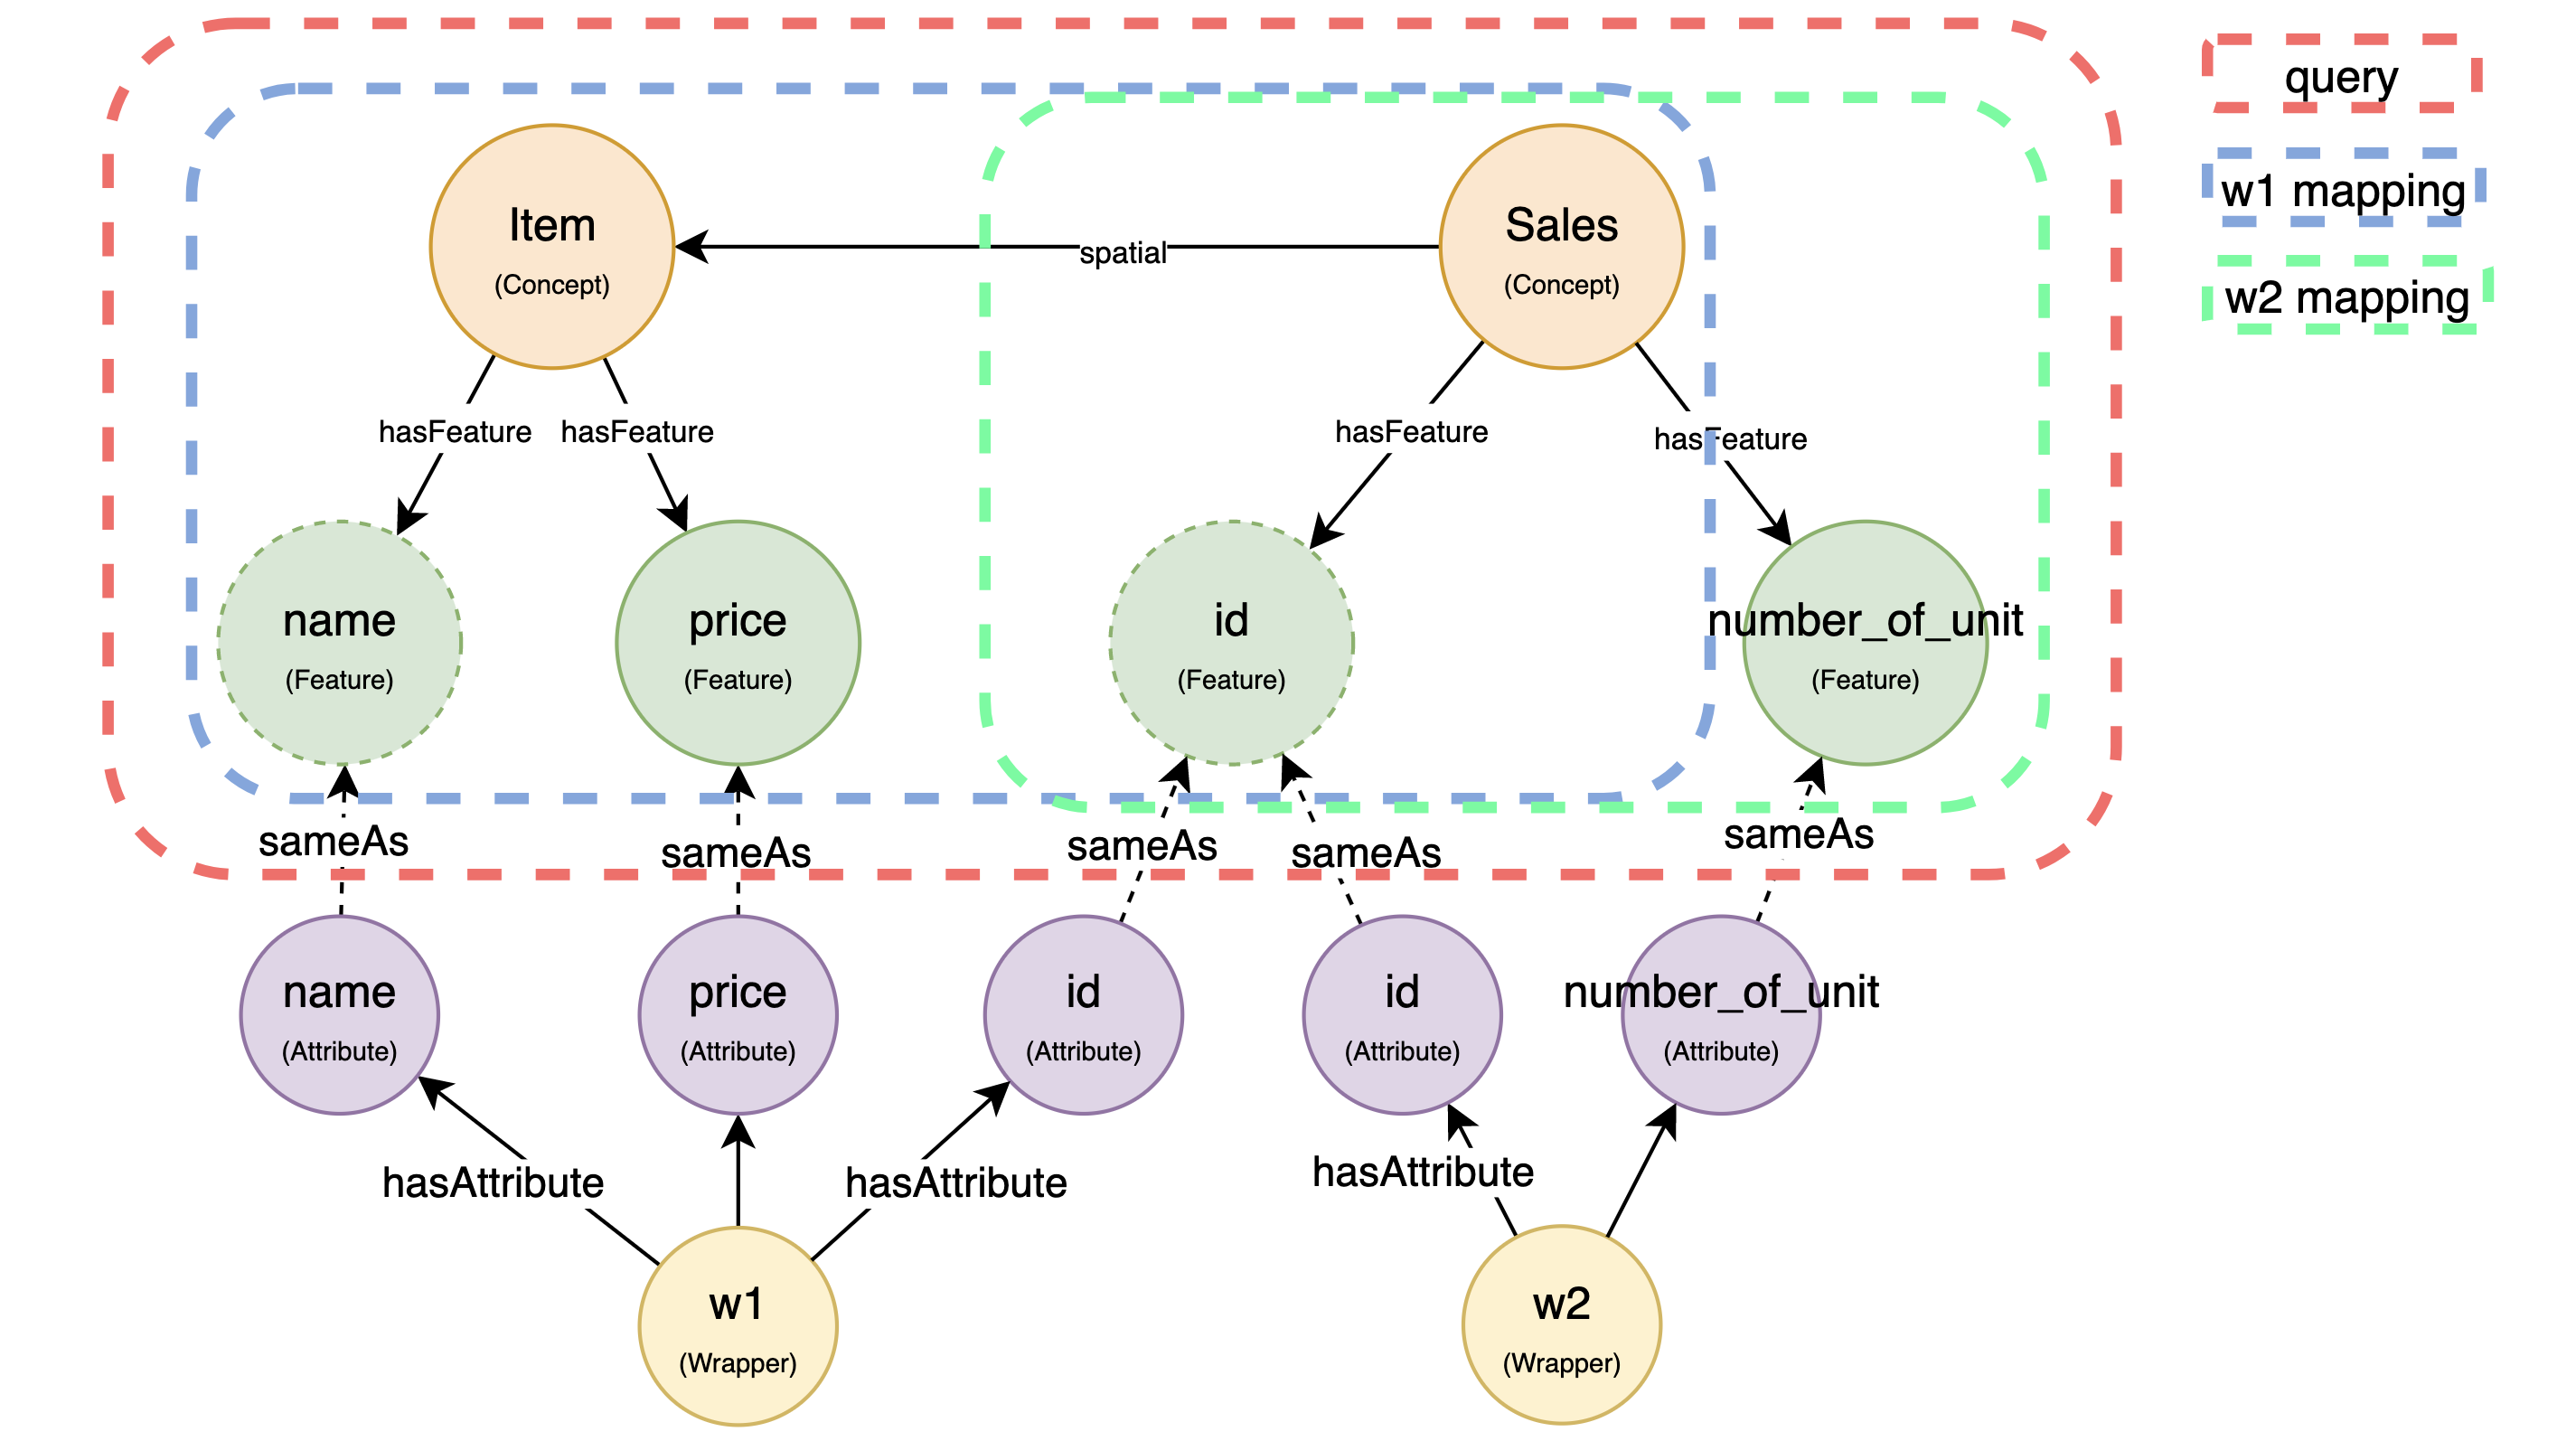
\includegraphics[width=\linewidth]{img/model.png}}
    \caption{A graphical representation of the graph model adopted by \systemName. The example depicts an integration graph $\integrationGraph$ related to sales, and a query $\globalQuery$ over $\targetGraph$ (the dashed red line), the LAV mapping of wrapper \textit{w1} (blue dashed line) and the LAV mapping of \textit{w2} (green dashed line).}
    \label{fig:Model}
\end{figure}
%

\begin{comment}
\section{Implicit Roll-Up model}
How do we want to design a multidimensional graph over \systemName\, model and syntax...


\begin{figure} [ht]
    \fbox{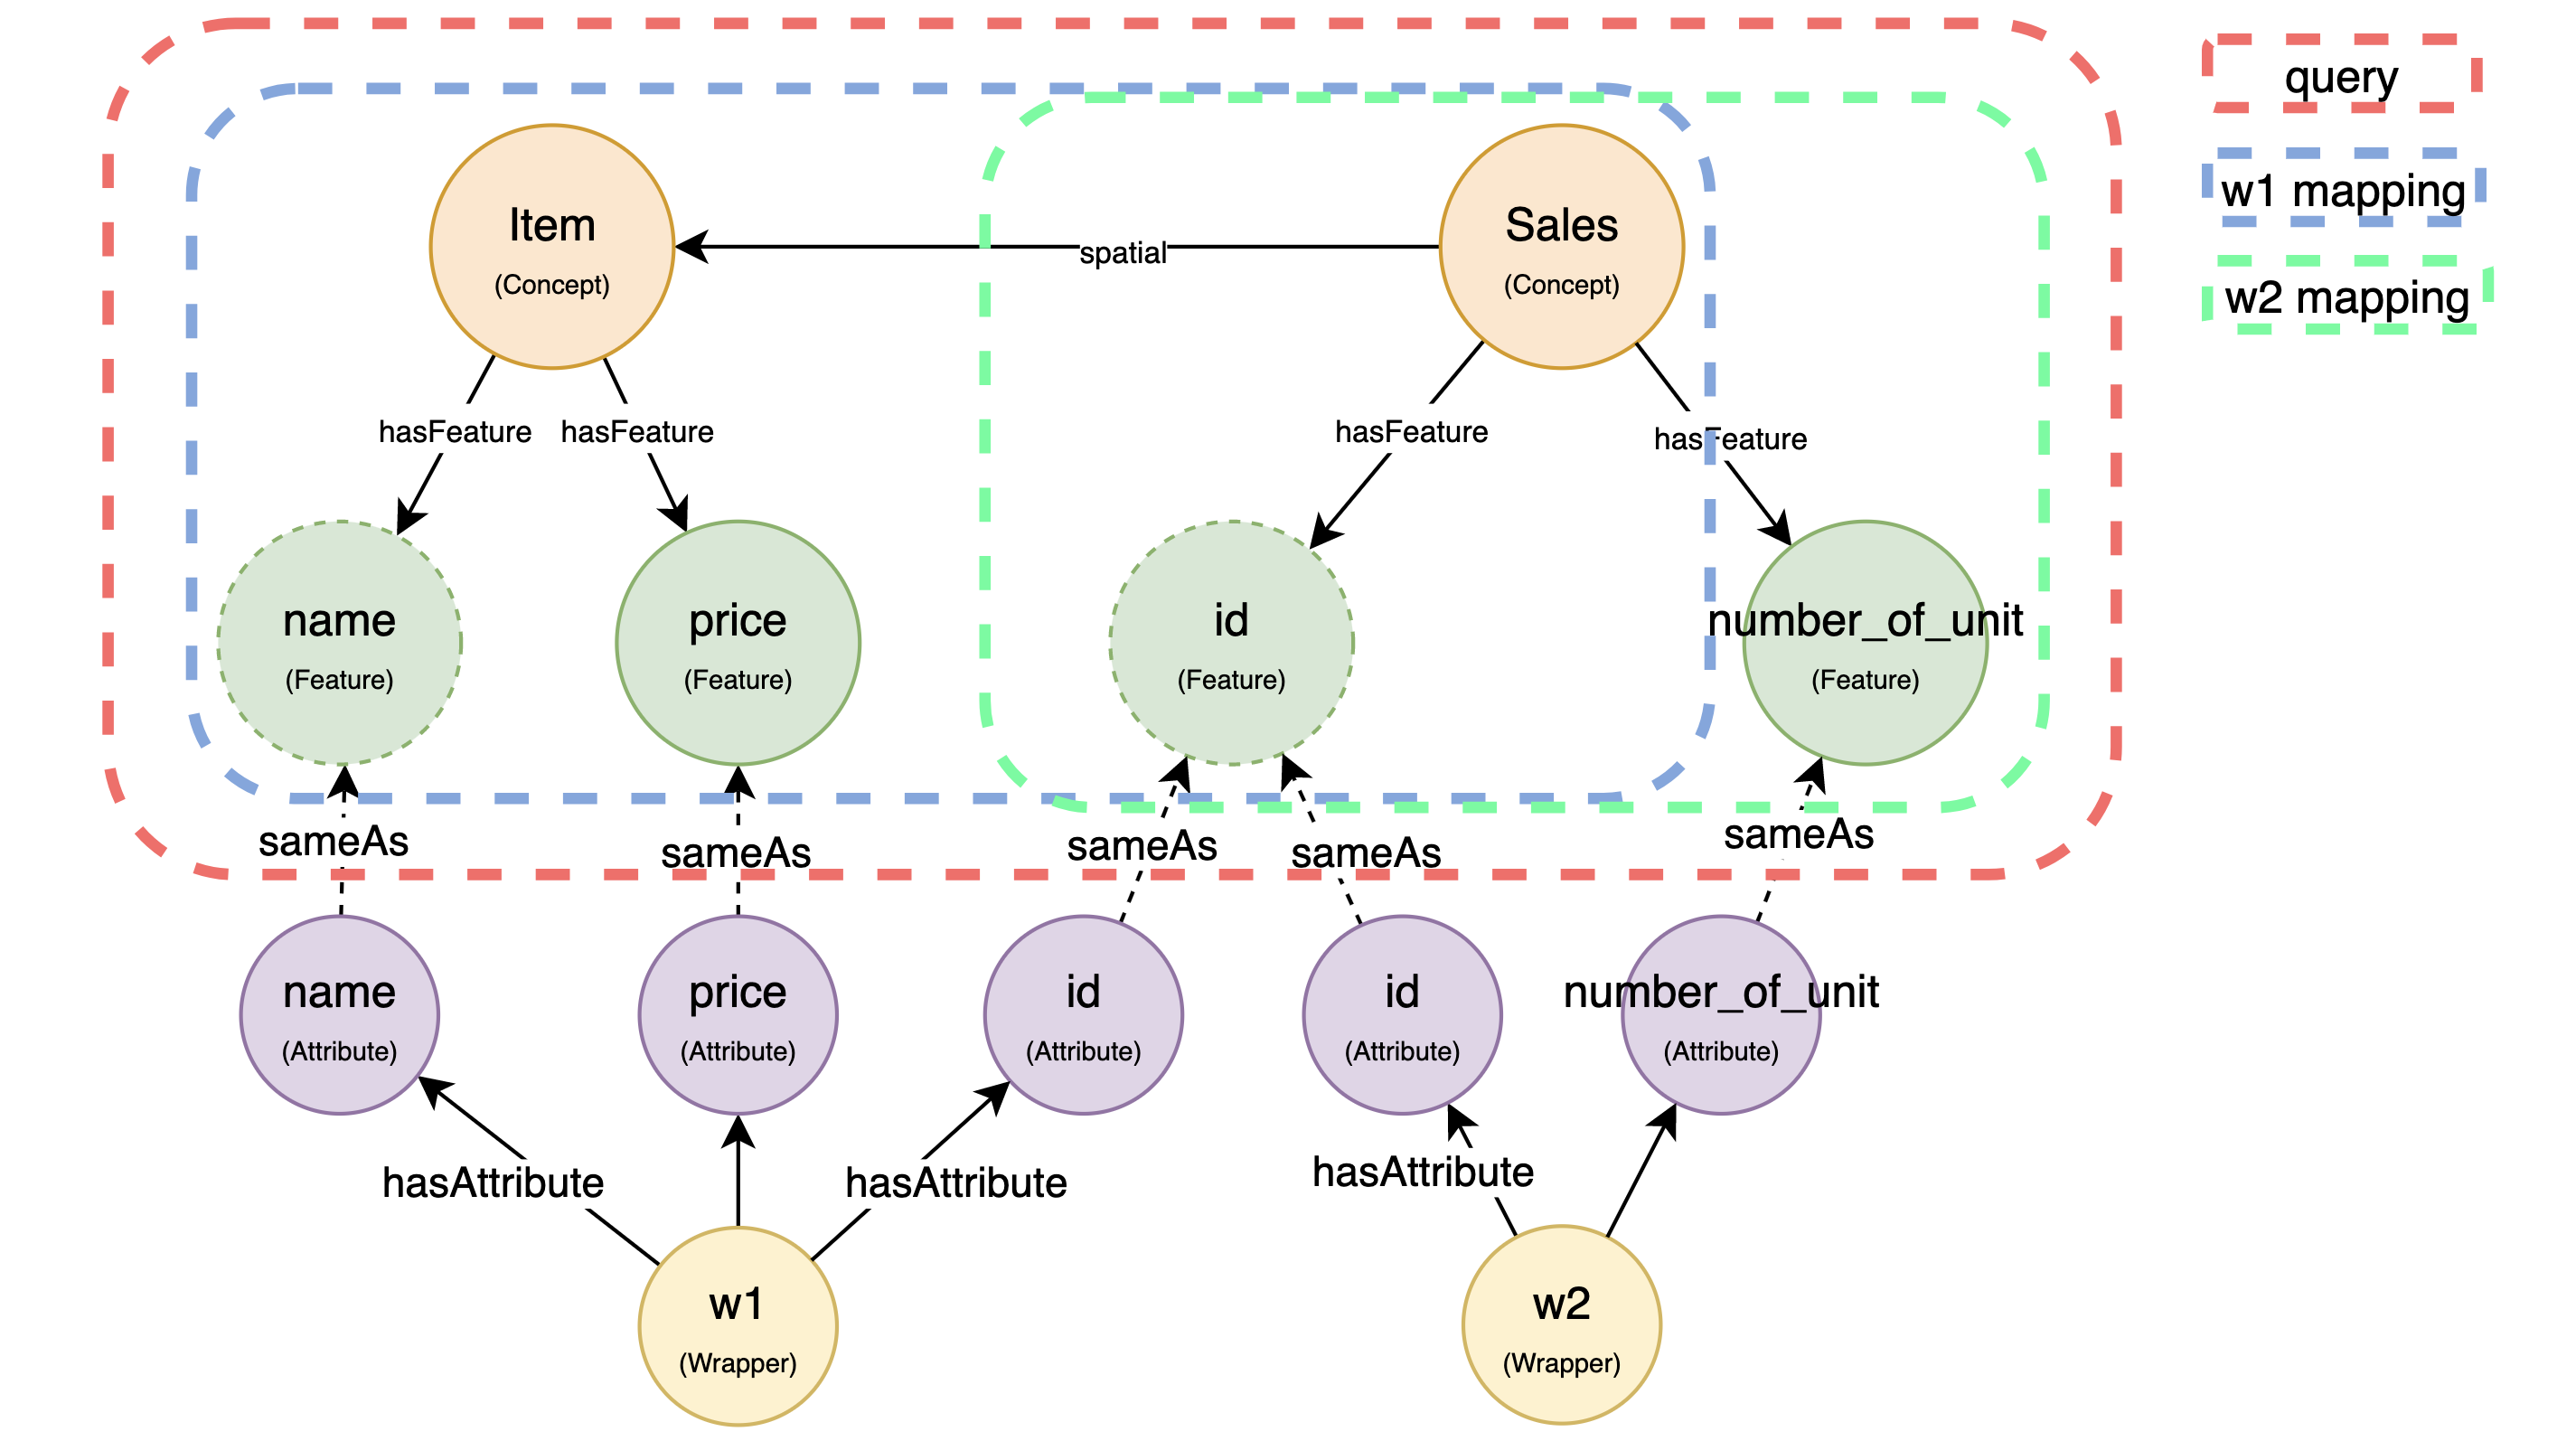
\includegraphics[width=\linewidth]{img/model.png}}
    \caption{The model.}
    \label{fig:Model}
\end{figure}
\end{comment}

\section{Joining dimensional data} \label{Joining dimensional data}
In this section we would like to introduce the intuition of how the join of dimensional data will be executed.
%
As we know this operation is very important for the Roll-Up since it will allow to rise up data at a lower granularity to the desired higher granularity and since this feature can actually already be achieved in \systemName\, this is why it will be explained into this chapter and not in the following one.
%
To execute the join of dimensional data it will be exploited the Rewriting Algorithm described in section \ref{Query answering}, since it will allow to execute join operations through different wrapper attributes.

The idea we got to solve this problem is using look-up tables to perform the join of dimensional data;
%
Look-up tables, that will be represented as wrappers, will lead the join operation between dimensions since, for each functional dependency, they will store how a level maps to the following higher granularity level.
%
This kind of approach, to work, will need a preliminary phase in which all the look-up table wrappers $\lut$ have to be loaded into the system, or linked to any multidimensional data repository, otherwise it will not be possible to execute the join and as consequence the Roll-Up.

Let's now start describing a how a dimension will be represented in \systemName\, with the help of Figure \ref{fig:Dimension}.
%
As in the multidimensional cube model $\multidimensionalCube$, where each dimension is divided in levels each one associated to an identifier, the same idea is replicated into the multidimensional graph $\multidimensionalGraph$.
%
Figure \ref{fig:Dimension} depicts a dimension with three level, as \textit{City}, \textit{Region} and \textit{Country}, each one linked to at least an identifier feature via \textit{hasFeature} relationship, respectively \textit{city}, \textit{region} and \textit{country}.
%
\begin{figure} [ht]
    \fbox{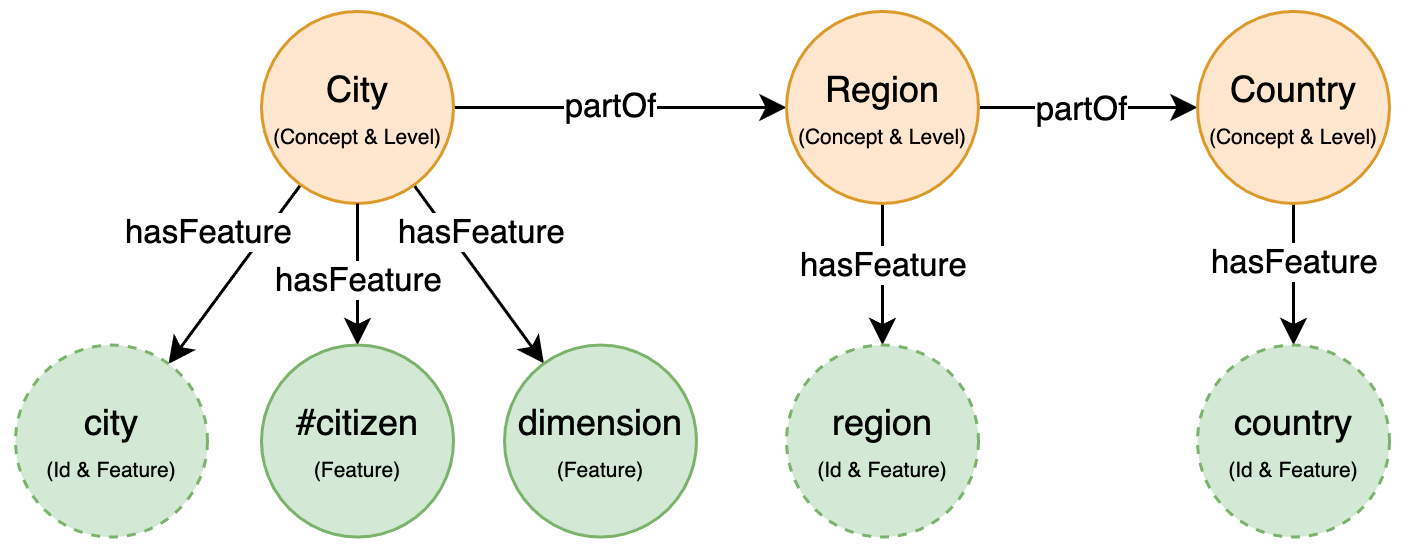
\includegraphics[width=\linewidth]{img/dimension.png}}
    \caption{How a dimensions will be represented over \systemName.}
    \label{fig:Dimension}
\end{figure}

Once explained how a dimension can be represented in $\multidimensionalGraph$ let's now go a bit ahead detailing how multidimensional data are joined \textbf{within} a dimension by means of the rewriting algorithm.
%
Figure \ref{fig:Join} depicts a very simple example of a multidimensional integration graph $\integrationGraph$, having on the right hand side $\multidimensionalGraph$ describing a dimension with two levels, and on the left hand side $\sourceGraph$ that contains wrappers and their attributes.
%
Also a visual query $\globalQuery$ over $\multidimensionalGraph$ is represented as a red dashed line.
%
We can see that three wrappers have been depicted in the figure, where \textit{w1} and \textit{w2} are regular data wrapper having a single attribute, respectively \textit{city} and \textit{country}, while the third wrapper \textit{w3} is a look-up table wrapper $\lut$ that will allow to join dimensional data.
%
In particular $\lut$ stores all the possible combination describing how each city can be converted into its respective a country.
%
Given a comprehensive query $\globalQuery$ that involves for a dimension, all the levels and the respective identifier feature, it will be possible to join all the levels queried with the higher granularity level if there is a $\lut$ bridging all the levels functional dependencies.
%
Finally the expected result from the execution of $\globalQuery$ with the rewriting algorithm would be the join between LAV mapping of \textit{w2},\textit{w3} (the look-up table) and \textit{w1}, having as result the following relational algebra expression.
\begin{equation} 
    \Uppi_{city,country}((w1\, \Bowtie_{city=city}\, w3)\, \Bowtie_{country=country}\, w1)
\end{equation}
%
\begin{figure} [ht]
    \fbox{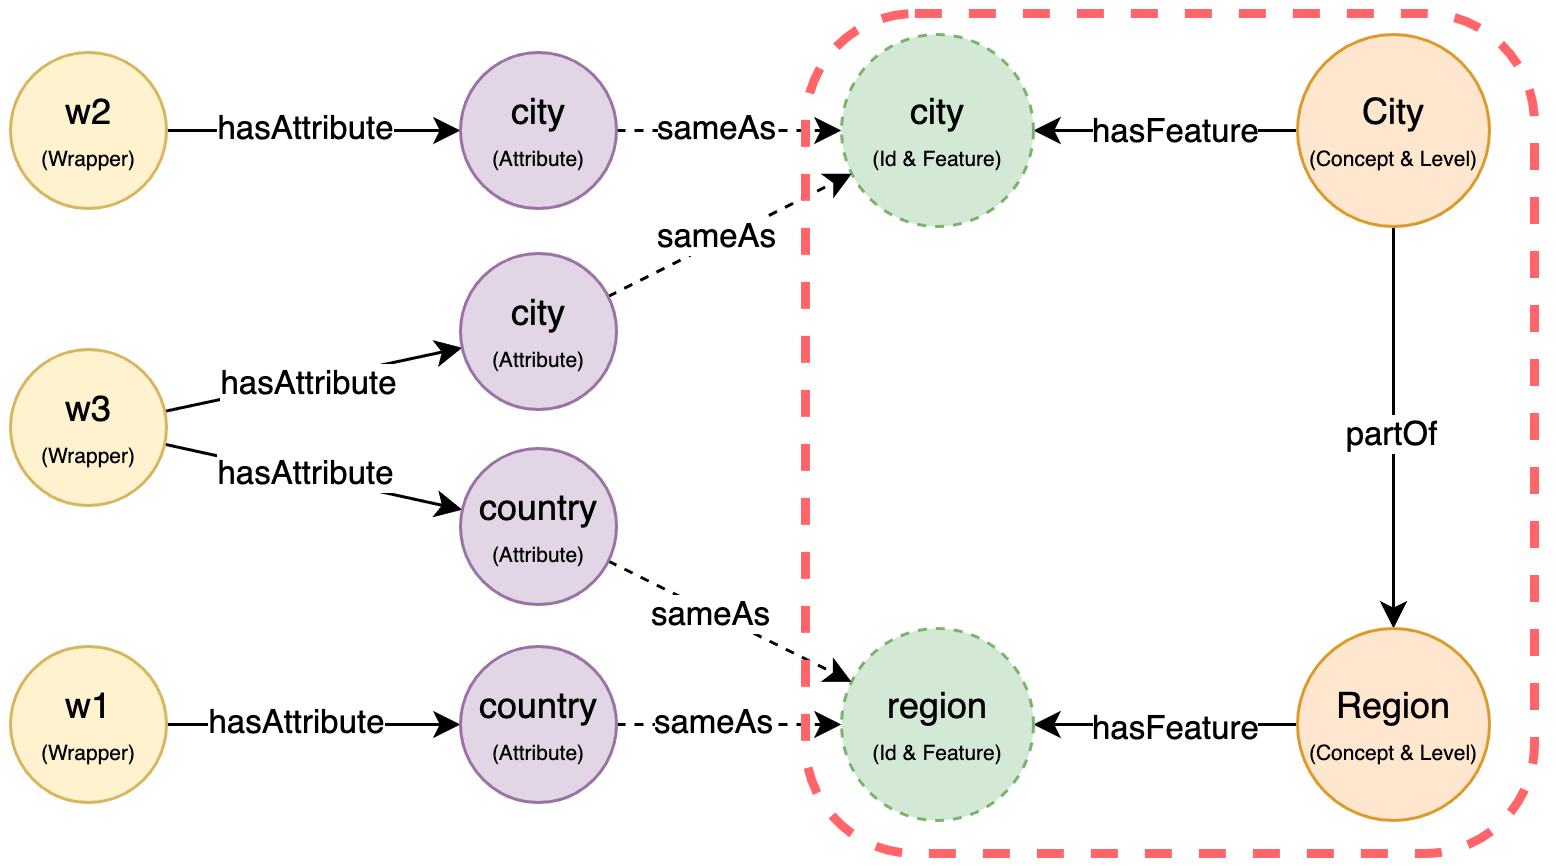
\includegraphics[width=\linewidth]{img/join.png}}
    \caption{How dimensional data are joined within a dimension over \systemName, where the dashed red line is a visual query $\globalQuery$.}
    \label{fig:Join}
\end{figure}
%

Let's now focus on the possible showcases of join \textbf{between} dimensions.
%
There are two main possible configuration of dimension representation wrapper side.
%
It is possible that each wrapper contains the entire  dimensional variables related to that observation, and it is actually the most likely scenario, but since the project is grounded in a data integration scenario, it may be also possible having disjointed dimensional data, each one exposed by a different wrapper but at the same time related to a single fact observation.
%
Figure \ref{fig:Join_2} is representing the first described scenario in which all the dimensional variable are represented inside just one wrapper (\textit{w1}).
%
This scenario is the easiest since it don't need the join of different dimensions variables and it will work over the assumptions we already did.
%
Given the queried feature \textit{region}, \textit{total revenue} and \textit{name}, the rewriting algorithm would return the data behaving to the wrappers having a LAV mapping (or join combination of mapping) where $\globalQuery$ is subsumed by the mapping.
%
\begin{figure} [ht]
    \fbox{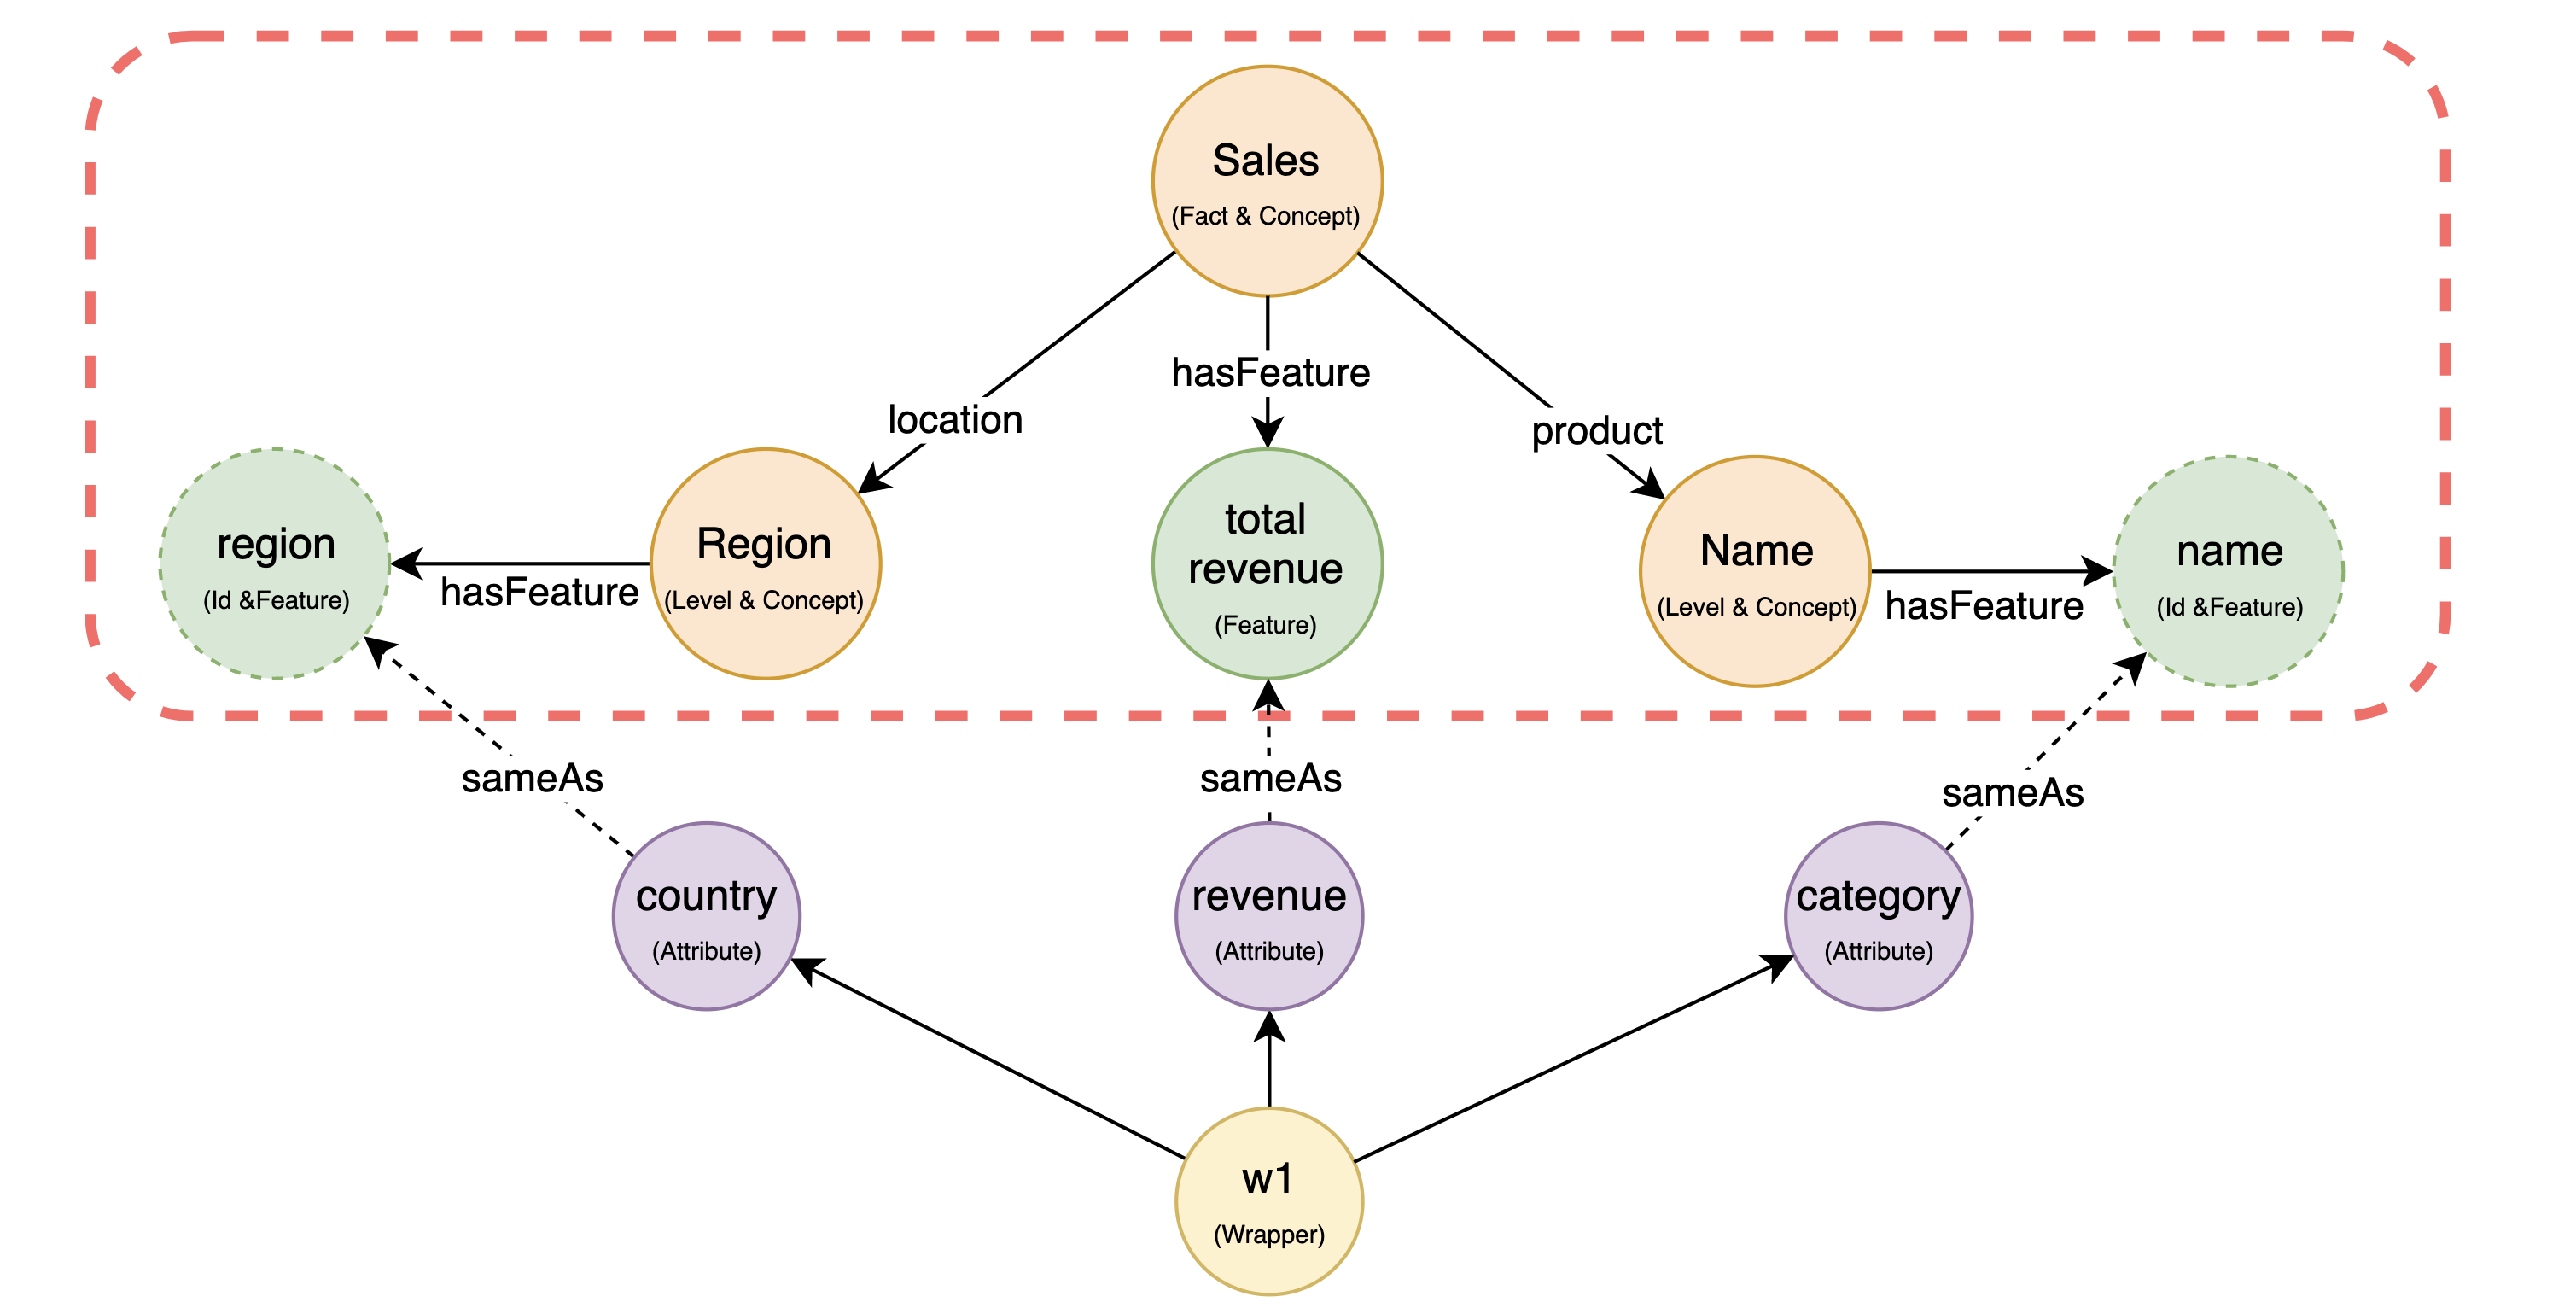
\includegraphics[width=\linewidth]{img/join_2.png}}
    \caption{Most likely scenario with all the dimensional variable contained in a single wrapper.}
    \label{fig:Join_2}
\end{figure}
%
In figure \ref{fig:Join_3}, as opposite, it is depicted the scenario in which different dimensions of a given fact are represented by means of separated wrappers.
%
In this case it is very important to adopt an identifier associated to the studied fact in order to correctly join separated dimensions having observations related to the same fact.
%
The identifier \textit{sale} will play this role.
%
\begin{figure} [ht]
    \fbox{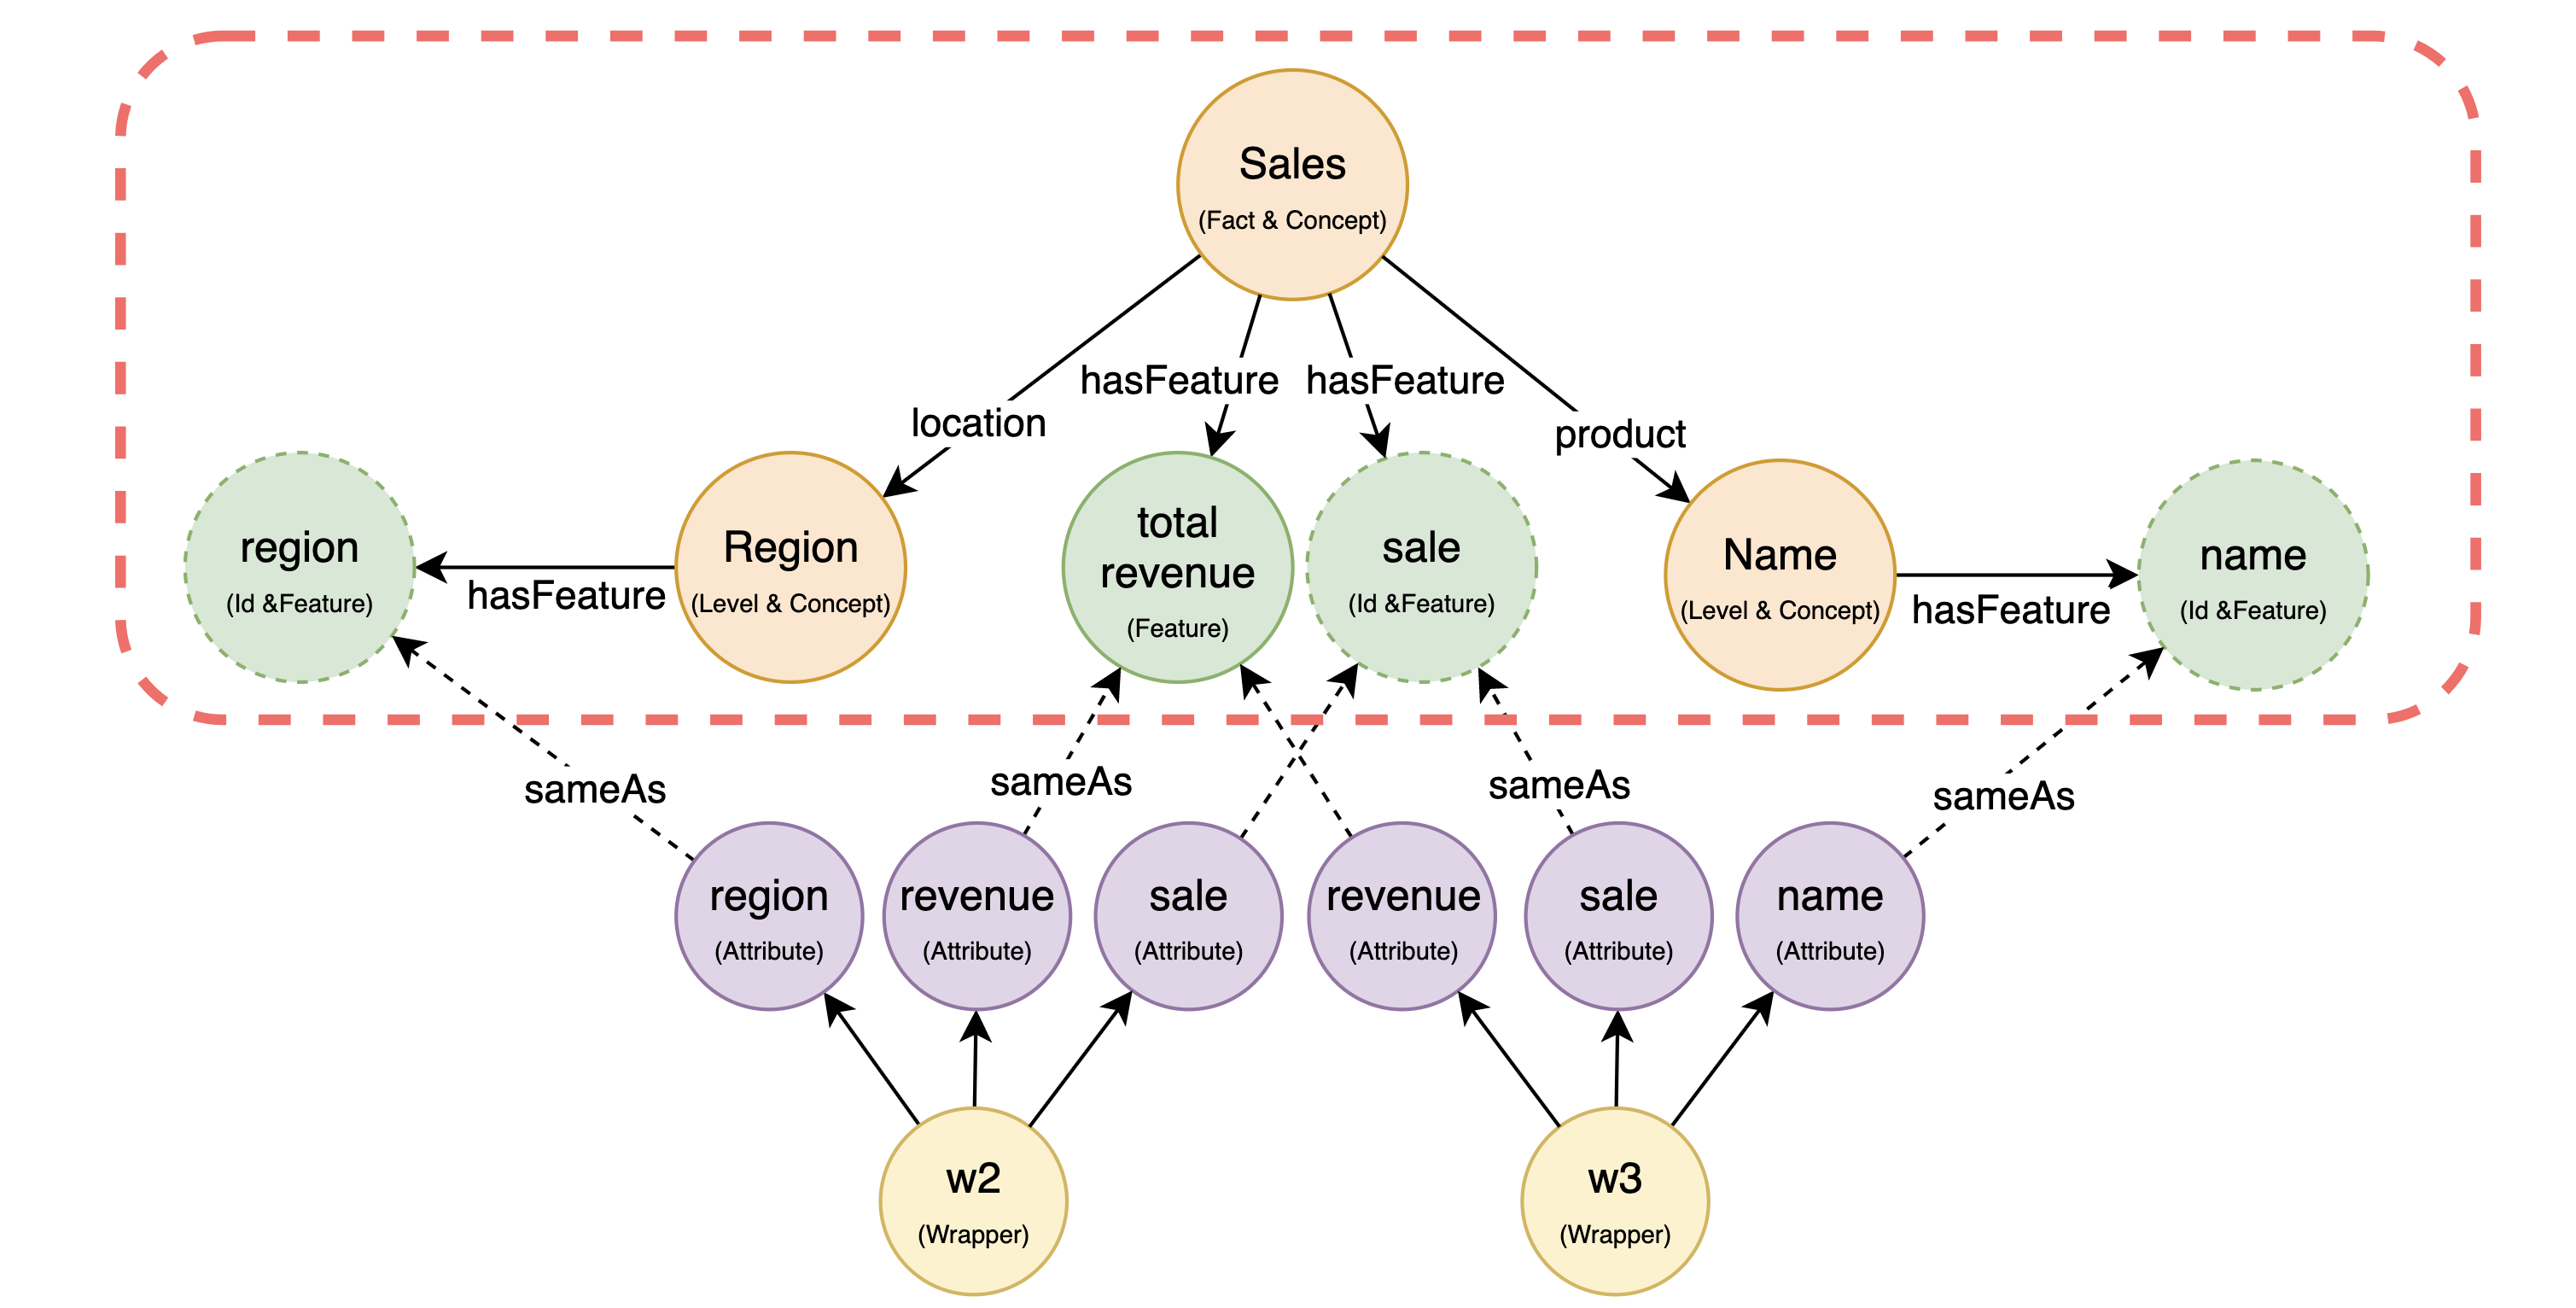
\includegraphics[width=\linewidth]{img/join_3.png}}
    \caption{Scenario with disjointed wrappers.}
    \label{fig:Join_3}
\end{figure}

\subsection{Aggregation function}
This section will show the intuition of how to include aggregation functions into \systemName.
%
Aggregation functions are very important to describe aggregation semantic of a queried feature.
%
In \systemName\, aggregations will be represented using the graph syntax, making pointing a vertex, with the semantic of an aggregation to a feature.
%
In Figure \ref{fig:Aggregations} have been depicted a clear example, having the feature \textit{number of unit} linked to an aggregating function \textit{Sum} and the feature \textit{total revenue} attached to an \textit{Avg} aggregating function.
%
\begin{figure} [ht]
    \fbox{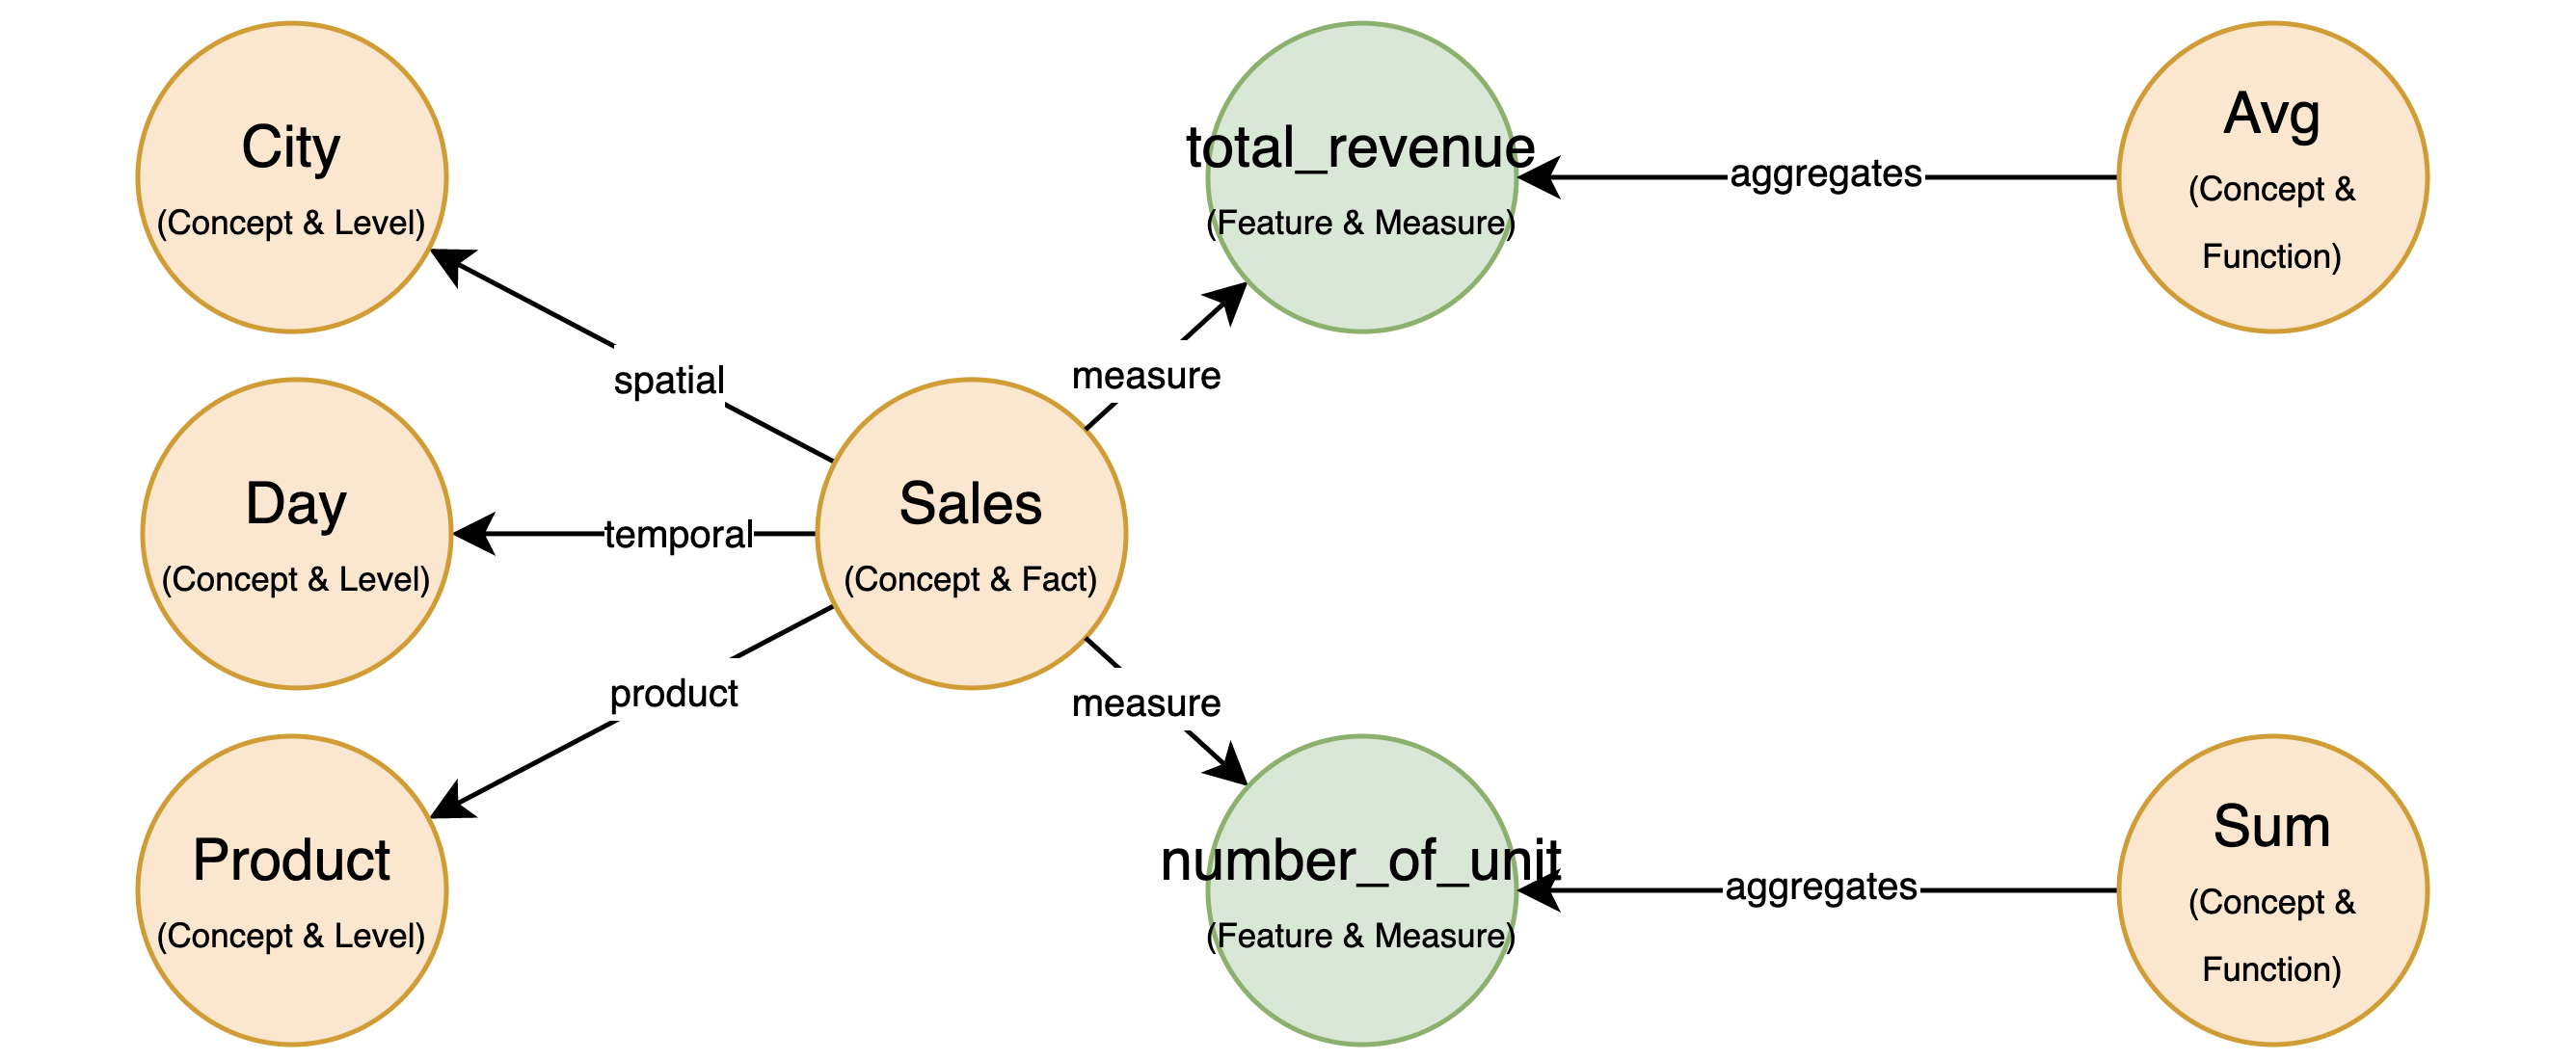
\includegraphics[width=\linewidth]{img/aggregations.png}}
    \caption{Example of aggregation functions \textit{Average} and \textit{Sum}.}
    \label{fig:Aggregations}
\end{figure}
%
It is very important having the aggregation functions represented into $\targetGraph$ and also $\multidimensionalGraph$ since being the Roll-Up performed implicit, it is important for the algorithm knowing the semantic of the aggregation.

\chapter{Description of the method}\label{Description of the method}

In this chapter it will be firstly described the model developed, aimed to support the operation of implicit Roll-Up and after it will follow a detailed explanation of the algorithm that will implement the implicit Roll-Up operation itself.
%
The model will extend the system \systemName\, defined in chapter \ref{Technology preliminaries}, and in particular, section \ref{Joining dimensional data} will be very important since it is the starting point of the reasoning behind the implicit Roll-Up algorithm, since it is related to the join of dimensional data.
%

\section{Preparation}
This section will formalise the two model $\multidimensionalCube$ and $\multidimensionalGraph$, showing and comparing the characteristics of each one.
%
Let's start defining a multidimensional cube $\multidimensionalCube$ as
\begin{equation}
    \fact \equiv \langle \dimension, \level, \measure, \levelsFundefinition, \partOfFunDefinition \rangle
\end{equation}
where $\fact$ is the described fact, $\dimension$ are all the multidimensional spaces known as dimensions, $\level$ are all the different granularity levels behaving to $\dimension$ and $\measure$ are all the study measures.
%
Finally we have $\levelsFunLabel$ and $\partOfFunLabel$ that are both functions.
%
The first, for a given $\dimension$, gets all the levels $\level$ behaving to $\dimension$ and the second describes all the functional dependencies between each level $\level$.
%
Let's now introduce the formalisation of multidimensional graph model $\multidimensionalGraph$ as follow.
%
\begin{equation}
\begin{split}
    \multidimensionalGraph \equiv \langle \fact, \dimension, \level, \measure, \aggregatingFunction, \dimensionsFundefinition, \measuresFunDefinition, \levelsFundefinition, \\\aggregatingFunctionDefinition, \partOfFunDefinition, \functionsFunDefinition\rangle
\end{split}
\end{equation}
%
Multidimensional graph model considers in addition the aggregating functions $\aggregatingFunction$, each one associated to a set of measures $\measure$ by the function $\aggregatingFunctionFunLabel$.
%
Aggregation functions in $\multidimensionalCube$ model are just related to the kind of measures subject to the Roll-Up operation, therefore the aggregating function is established run time, while in $\multidimensionalGraph$ model it needs to be "hard-coded" into the schema in order to perform implicit Roll-Up, since being the operation performed implicitly, it will not be possible to choose it while executing the query.
%
$\multidimensionalGraph$ model can also describe more then one fact while $\multidimensionalCube$ model describes just one.
%
That's why $\multidimensionalGraph$ model have a function $\dimensions$ that for a given fact $\fact$ gets a set of dimensions behaving to $\fact$, and for the same reason there is also a set of measures related to $\fact$ by the function $\measuresFunLabel$ and finally a function $\functionsFunLabel$ that shows all the $\aggregatingFunction$ associated to a given $\fact$.
%
Another important difference between $\multidimensionalCube$ and $\multidimensionalGraph$ is that the latter, as $\targetGraph$, is clearly graph based and it deals with triples (e.g. it is described with a set of triples).
%
From now on it will be introduced the triple notation behind each element of $\multidimensionalGraph$ relying to the triple syntax introduced in section \ref{GFDM model}.
%
The following definitions will refer to the Figure \ref{fig:running_example}.
%
\begin{figure} [ht]
    \fbox{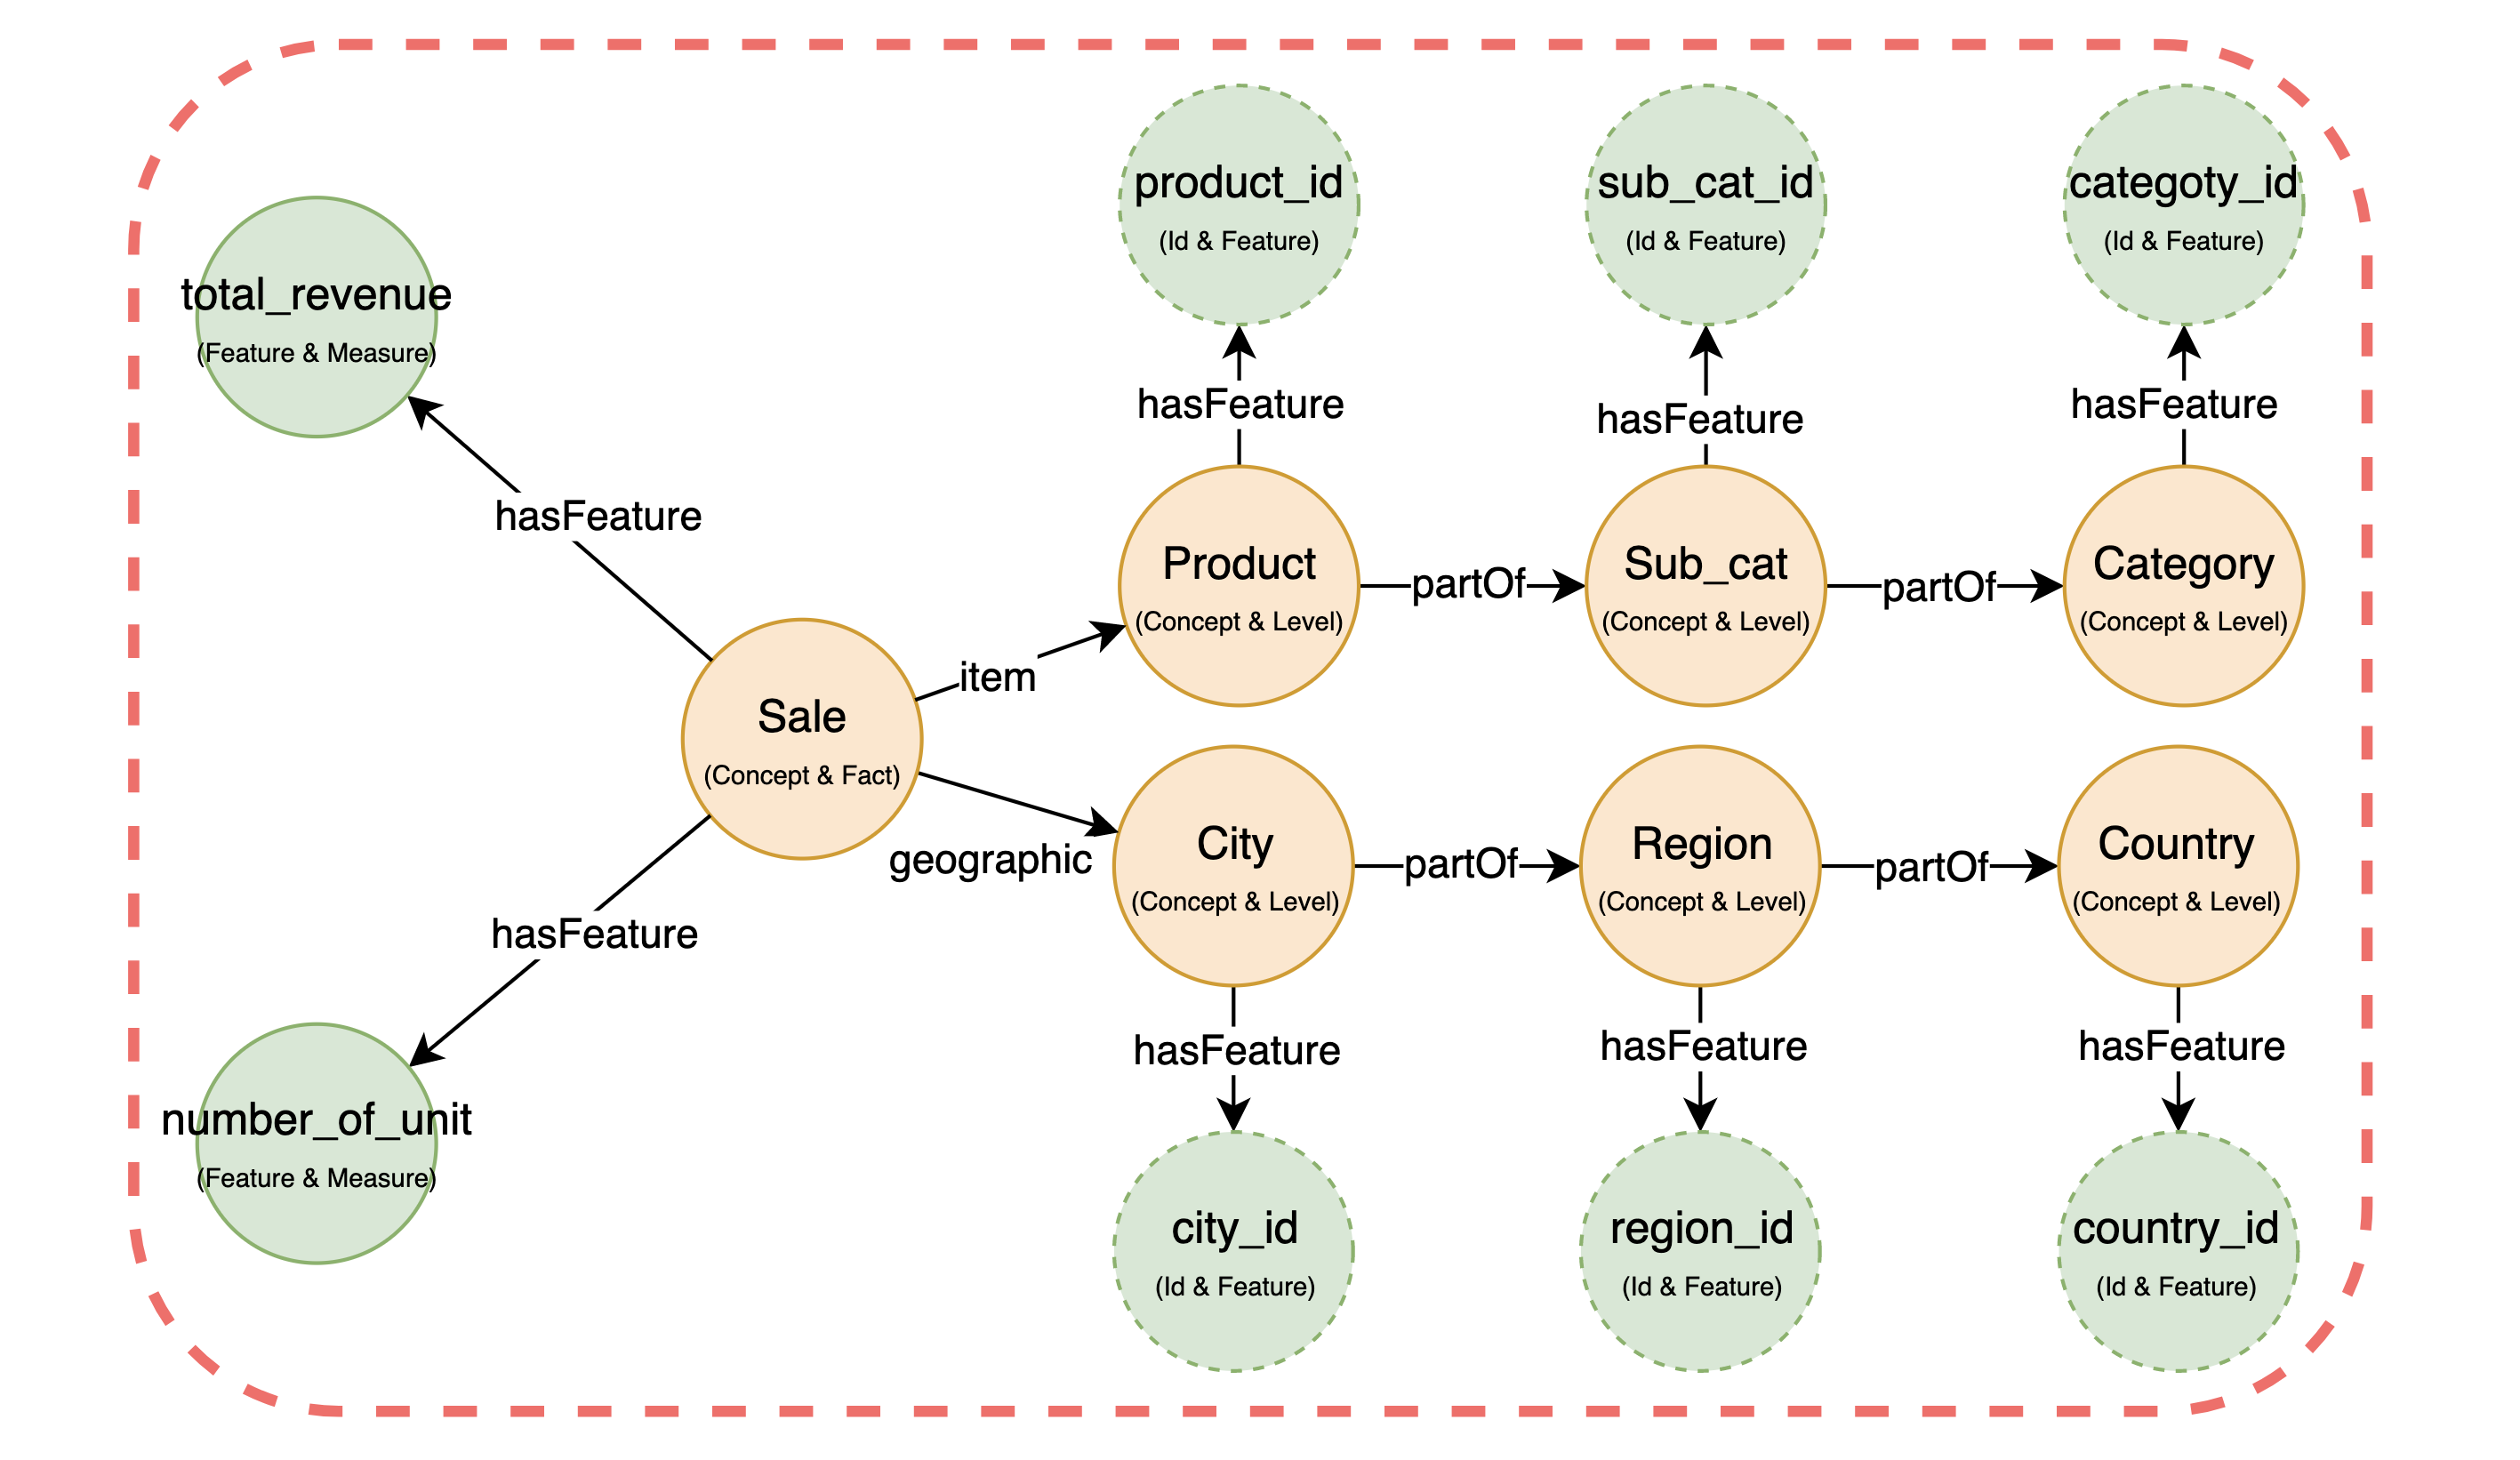
\includegraphics[width=\linewidth]{img/running_example.png}}
    \caption{Running example, where the dashed red line is the query triggered.}
    \label{fig:running_example}
\end{figure}

Let's now formalise the triple notation of $\multidimensionalGraph$ as the union of a set of fact $\set{\fact}$, a set of aggregation functions $\set{\aggregatingFunction}$ and the $\targetGraph$ that is a set of triples as well.
%
\begin{equation}
    \triple{\multidimensionalGraph} \equiv \set{\triple{\fact}} \cup \triple{\targetGraph} \cup \set{\triple{\aggregatingFunction}}
\end{equation}
\begin{equation}
    \triple{\targetGraph} \sqsubseteq \triple{\multidimensionalGraph} \sqsubseteq \triple{\integrationGraph}
\end{equation}

Introduce now the triple notation for a dimension $\dimension$, given as the union of all the $\partOfFunLabel$ relationship triples in $\dimension$, referring to the example we have $\set{City,\partOfFunLabel,Region}$ and $\set{Region,\partOfFunLabel,Country}$ and the union of also all the triples $hasFeature$ defining each level $\idFeature$, then $\set{City,hasFeature,city\_id}$, $ \set{Region,hasFeature,region\_id} $ and $\set{Country,hasFeature,country\_id}$.
%
Formally the triples involving $\dimension$ are given by the following statements.
%
\begin{equation}
    \set{\level}_{\dimension} \equiv \levels(\dimension) \equiv \{\level_{0},...,\level_{size(\levels(\dimension)) - 1}\}
\end{equation}
%
\begin{equation}
    \triple{hasFeature} \equiv \cup_{i = 0}^{size(\set{\level}_{\dimension}) - 1} \langle \level_{i}, hasFeature, \id(\level_{i}) \rangle
\end{equation}
%
\begin{equation}
    \triple{\partOfFunLabel} \equiv \cup_{i = 0}^{size(\set{\level}_{\dimension}) - 2} \langle \level_{i}, \partOfFunLabel, \partOfFunLabel(\level_{i}) \rangle
\end{equation}
%
\begin{equation}
    \triple{\dimension} \equiv \triple{\partOfFunLabel} \cup \triple{hasFeature}
\end{equation}
%

The triple notation for a fact $\fact$ is defined as the union of all the dimensions behaving to $\fact$, as $\triple{\dimension}$ (that have been defined right before) given by $\triple{\dimensions(\fact)}$.
%
For the fact \textit{Sale} there will be all the triple related to the geographic and also the item dimensional space.
%
Then will have to be considered the triple connecting the fact to each lower granularity level of dimensions, as $\set{Sale,item,Product}$ and $\set{Sale,geographic,City}$.
%
Also all the triples defining the measures $\measure$ that behave to the $\fact$ have to be considered, such as $\set{Sale,hasFeature,total\_revenue}$ and $\set{Sale,hasFeature,number\_of\_unit}$.
%
Since we want as goal to keep flexibility to the system, both the paths that links $\fact$ to $\measure$ and $\dimension$ don't have to be necessarily directed therefore to define the predicate $\predicate$ will be used regular expressions in the form of $\predicate^{+}$ to define flexible paths.
%
Then the triple notation of $\fact$ can be stated as follow.
%
\begin{equation}
    \set{\dimension}_{\fact} \equiv \dimensions(\fact) \equiv \{\dimension_{0},...,\dimension_{size(\dimensions(\fact)) - 1}\}
\end{equation}
%
\begin{equation}
    \set{\measure}_{\fact} \equiv \measures(\fact) \equiv \{\measure_{0},...,\measure_{size(\measures(\fact)) - 1}\}
\end{equation}
%
\begin{equation}
    \triple{dimLabels} \equiv \cup_{i = 0}^{size(\set{\dimension}_{\fact}) - 1} \set{\fact,\predicate^{+},lowerGranularityLevel(\dimension_{i})}
\end{equation}
%
\begin{equation}
    \triple{measuresLabels} \equiv \cup_{i = 0}^{size(\set{\measure}_{\fact}) - 1} \set{\fact,\predicate^{+},\measure_{i}}
\end{equation}
%
\begin{equation}
    \triple{\fact} \equiv \triple{\set{\dimension}_{\fact}} \cup \triple{dimLabels} \cup \triple{measuresLabels}
\end{equation}
%
It is also important to state the relationship between $\triple{\dimension}$, $\triple{\fact}$ and $\triple{\multidimensionalGraph}$ having the following rule.
%
\begin{equation}
    \triple{\dimension} \sqsubseteq \triple{\fact} \sqsubseteq \triple{\multidimensionalGraph}
\end{equation}
%
Let's finally see the triple notation for an aggregating function, having all the triple connecting the function to the referred measure.
%
Consider that is possible having one $\aggregatingFunction$ linked to one or more $\measure$.
%
Referring to the running example let's suppose there are two aggregating function \textit{sum} and \textit{avg}, respectively aggregating \textit{number\_of\_unit} and \textit{total\_revenue}, then there will be the following two triples $\set{sum,\aggregatingFunctionFunLabel,number\_of\_unit}$ and $\set{avg,\aggregatingFunctionFunLabel,total\_revenue}$.
%
\begin{equation}
    \set{\aggregatingFunction}_{\multidimensionalGraph} \equiv \functionsFunLabel(\multidimensionalGraph) \equiv \{\aggregatingFunction_{0},...,\aggregatingFunction_{size(\functionsFunLabel(\multidimensionalGraph)) - 1}\}
\end{equation}
%
\begin{equation}
    \set{\measure}_{\aggregatingFunction_{i}} \equiv \aggregatingFunctionFunLabel(\aggregatingFunction_{i}) \equiv \{\measure_{0},...,\measure_{size(\aggregatingFunctionFunLabel(\aggregatingFunction_{i})) - 1}\}
\end{equation}
%
\begin{equation}
    \triple{\aggregatingFunction} \equiv \cup_{i = 0}^{size(\set{\aggregatingFunction}_{\multidimensionalGraph}) - 1} \cup_{j = 0}^{size(\aggregatingFunctionFunLabel(\aggregatingFunction_{i})) - 1} \set{\aggregatingFunction_{i}, \aggregatingFunctionFunLabel,\aggregatingFunctionFunLabel(\aggregatingFunction_{i})_{j}}
\end{equation}

Let's consider now the querying for $\multidimensionalGraph$, where $\globalQuery$ is a pattern matching or visual query over $\multidimensionalGraph$ and $\sqlQuery$ is a query in SQL format.
%
Introduce also the concept of dimension query $\dimensionQuery$.
%
A dimension query is a sub-graph of a given $\dimension$ in $\globalQuery$ and its purpose is to allow to join dimensional data at low level granularity rising them to the required higher granularity asked by $\globalQuery$ through $\lut$ (described in section \ref{Joining dimensional data}).
%
An example of dimension queries for the running example have been depicted in Figure \ref{fig:dimension_queries} containing all the dimension queries for the product and  geographical dimension.
%
\begin{figure} [ht]
    \fbox{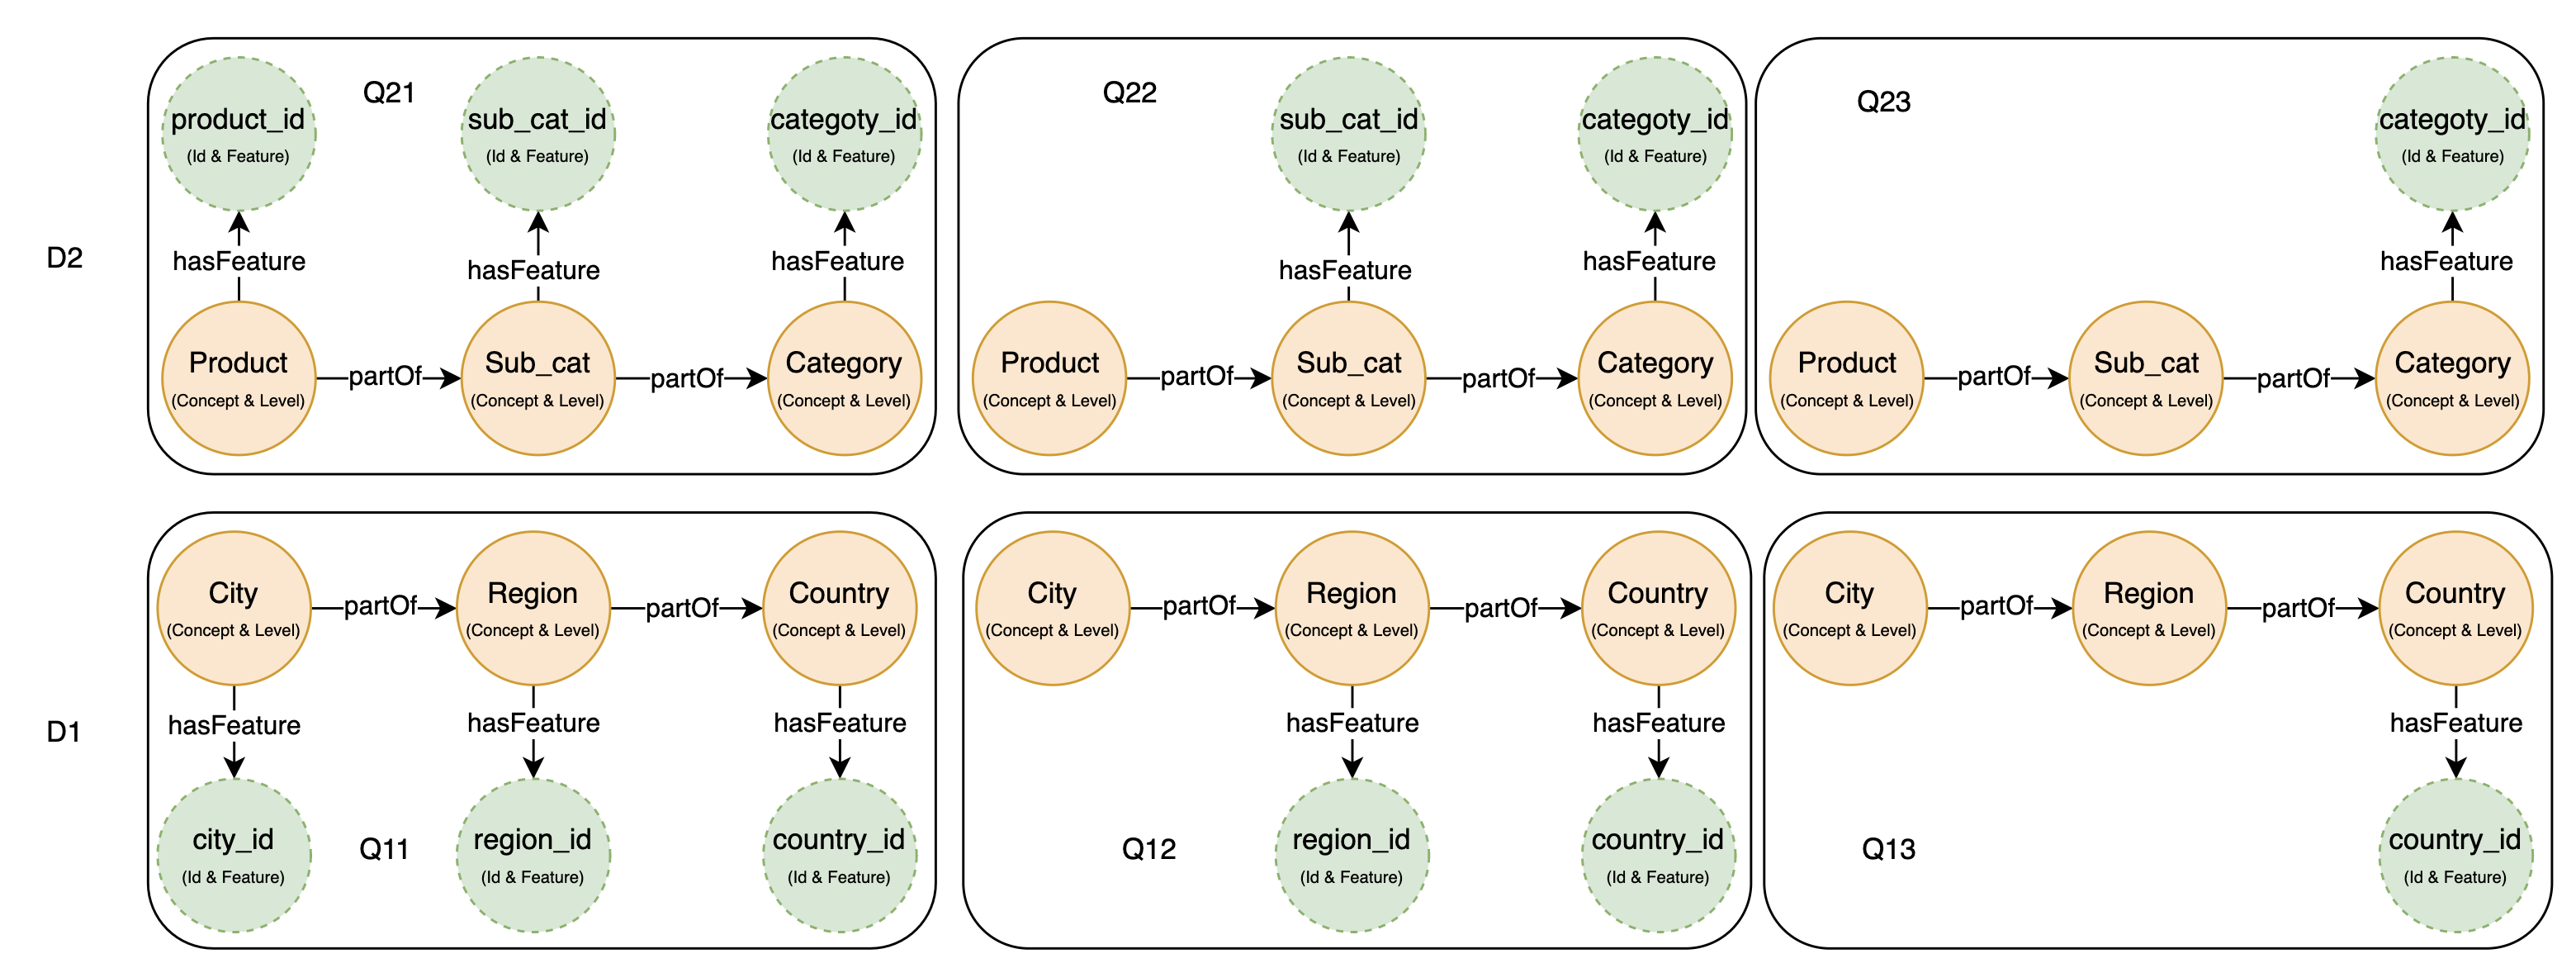
\includegraphics[width=\linewidth]{img/dimensionQueries.png}}
    \caption{Dimension queries $\dimensionQuery$ for product and  geographical dimension.}
    \label{fig:dimension_queries}
\end{figure}
%
Let's take as example the dimension queries for the geographical dimension \textit{D1} in Figure \ref{fig:dimension_queries}.
%
The queried granularity in $\globalQuery$ in the running example is \textit{Country} since it is the higher granularity level that contains the identifier.
%
Then what we would like to achieve is to include in the query result all the data at \textit{Country} granularity (\textit{Q13}), the data at \textit{Region} granularity joined with the relative \textit{Country} (\textit{Q12}) and also the data at \textit{City} granularity joined firstly with \textit{Region} and finally with \textit{Country} (\textit{Q11}).
%
The number of dimension query for each dimension and the total number of dimension queries will be the following.
%
\begin{equation}
    \set{\dimension}_{\globalQuery} \equiv \dimensions(\globalQuery) \equiv \{\dimension_{0},...,\dimension_{size(\dimensions(\globalQuery)) - 1}\}
\end{equation}
%
\begin{equation}
    cardinality(\dimensionQuery_{i}) \equiv size(\levels(\dimension_{i}))
\end{equation}
%
\begin{equation}
    cardinality(\dimensionQuery) \equiv \sum_{i=0}^{size(\dimensions(\globalQuery)) - 1} cardinality(\dimensionQuery_{i})
\end{equation}
%
A Roll-Up query is a sub-set of $\globalQuery$ and it is a $\globalQuery$ that has as dimension one possible combination of the dimension queries (e.g. one entry of the Cartesian Product of dimension queries).
%
Referring to the Figure \ref{fig:roll-up-query}, there are nine possible combination of Roll-Up query, given by $\{Q21, Q22, Q23\} \times \{Q11, Q12, Q13\}$.
%
The number of the Roll-Up queries for $\globalQuery$ is given by the following formula.
%
\begin{equation}
    \set{\dimension}_{\globalQuery} \equiv \dimensions(\globalQuery) \equiv \{\dimension_{0},...,\dimension_{size(\dimensions(\globalQuery)) - 1}\}
\end{equation}
%
\begin{equation}
    cardinality(\rollUpQuery) \equiv \prod_{i=0}^{size(\set{\dimension}_{\globalQuery}) - 1} cardinality(\dimensionQuery_{i})
\end{equation}
%
\begin{figure} [ht]
    \fbox{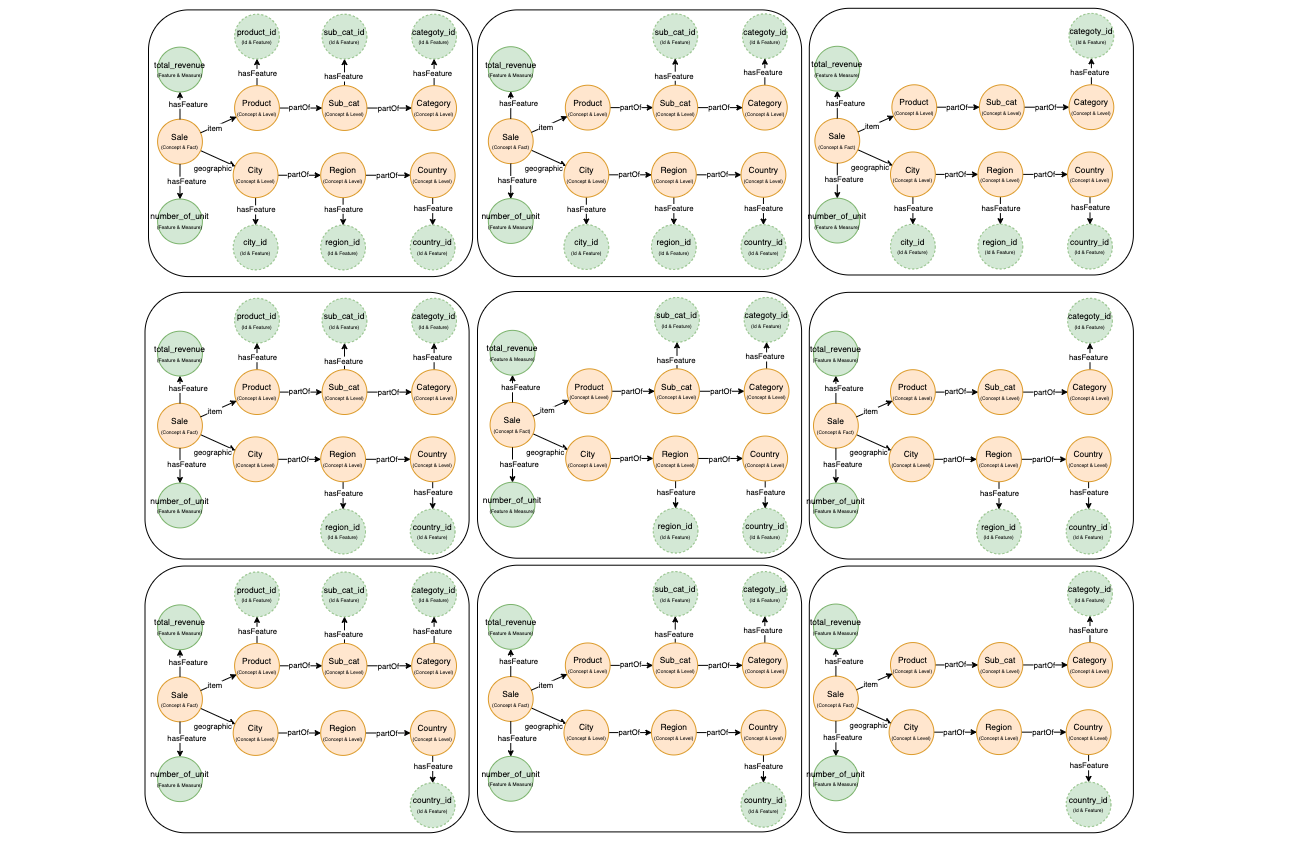
\includegraphics[width=\linewidth]{img/rollUpQuery.png}}
    \caption{All the Roll-Up queries for $\globalQuery$.}
    \label{fig:roll-up-query}
\end{figure}

Queries have also their triple notation and it is the following.
%
\begin{equation}
    \triple{\dimensionQuery} \sqsubseteq \triple{\dimension}
\end{equation}
%
\begin{equation}
    \triple{\dimensionQuery} \sqsubseteq \triple{\rollUpQuery} \sqsubseteq \triple{\globalQuery} \sqsubseteq \triple{\targetGraph} \sqsubseteq \triple{\multidimensionalGraph}
\end{equation}

The connections between $\targetGraph$ and $\multidimensionalGraph$ is done generating taxonomies between $\targetGraphVertex$ and $\targetGraphEdge$, and $\targetMultidimensionalGraphVertex$ and $\targetMultidimensionalGraphEdge$, and the relationships are the following; 
\begin{equation}
    \level \land \aggregatingFunction \sqsubseteq \concept \sqsubseteq \targetMultidimensionalGraphVertex
\end{equation}
\begin{equation}
    \measure \sqsubseteq \feature \sqsubseteq \targetMultidimensionalGraphVertex
\end{equation}
\begin{equation}
    \partOfFunLabel \land \aggregatingFunctionFunLabel \sqsubseteq \targetMultidimensionalGraphEdge
\end{equation}

Let's finally also introduce some simple functions that are $traverses$ over $\multidimensionalGraph$ that will be very useful in the next section for the execution of the algorithm; 
%
$\measures(\targetGraph^{+})$, $\features(\targetGraph^{+})$, $\levels(\targetGraph^{+})$, $\dimensions(\targetGraph^{+})$ are respectively all the measures $\measure$, features $\feature$, levels $\level$ and dimensions $\dimension$ in a given $\targetGraph$, that means that those function can be both called on $\globalQuery$ and $\multidimensionalGraph$.
%
Also $\id(\concept)$ are all the $\idFeature$ for a given $\concept$.
%
The functions $ \lowerGranularityLevel $ and $ \higherGranularityLevel $ as respectively the lower granularity $\level$ and the higher granularity $\level$ of a given dimension $\dimension$, holding the relationship $\set{\level,hasFeature,\id(\level)}$ (e.g. the higher or lower granularity level should be linked to an $\idFeature$).
%
Finally the function $\aggregatingFunctions(\multidimensionalGraph)$ will describe all the aggregating functions $\aggregatingFunction$ in $\multidimensionalGraph$.
%

\section{The Implicit Roll-Up algorithm} \label{Implicit RollUp}
In this section it will follow up a detailed explanation of the algorithm developed to perform implicit Roll-Up.
%
The $traverses$ defined before will be massively used to simplify the understandability of the algorithms but their implementation will not be detailed since it is very related to the implementation technique.
%
The main flow have been depicted in the Algorithm \ref{alg:implicitRollUp}, where it is clear which are the main steps of the algorithm and how they are related to each other.
%
The algorithm will take as input the multidimensional graph $\multidimensionalGraph$, the global query $\globalQuery$ and the function $rewrite$ that will execute underneath the rewriting algorithm and finally it will generate a SQL view $\sqlQuery$.
%
The function $rewrite$ takes as argument two queries, $\globalQuery$ and $\globalQuery_{min}$ executing $\globalQuery$ with the respect of the \textit{minimal} property according to $\globalQuery_{min}$.
%
As output $implicitRollUp$ will generate a complex SQL query $\sqlQuery$ given by the union of multiple call of $rewrite$ if $\globalQuery$ has an aggregation semantic.
%
If any aggregation semantic is detected in $\globalQuery$ the output of the algorithm will be just the execution of $rewrite$ over $\globalQuery$.
%
\begin{algorithm}[ht]
\caption{implicitRollUp}\label{alg:implicitRollUp}
\textbf{Input:} $\multidimensionalGraph,\globalQuery,rewrite:(\globalQuery,\globalQuery_{min}) \rightarrow \sqlQuery$\\
\textbf{Output:} $\sqlQuery$
\begin{algorithmic}[1]
\If{$canAggragate(\globalQuery)$}
    \State $\set{\level} \gets extractGroupByClauses(\globalQuery)$
    \State $\langle \aggregatingFunction,\langle \measure \rangle \rangle \gets extractAggregationClauses(\multidimensionalGraph,\globalQuery)$
    \State $\set{\level}_{sql} \gets parseGroupByClauses(\set{\level})$
    \State $\langle \aggregatingFunction,\langle \measure \rangle \rangle_{sql} \gets parseAggregationClauses(\langle \aggregatingFunction,\langle \measure \rangle \rangle)$
    \State $\set{\dimension, \set{\dimensionQuery}} \gets generateDimensionQueries(\globalQuery,\multidimensionalGraph)$
    \State $\set{\globalQuery_{rollUp}} \gets crossProductUnion(\globalQuery,\set{\dimension, \set{\triple{\dimension}}})$
    \State $\set{\sqlQuery} \gets rewriteAll(rewrite,prune(\globalQuery))(\set{\globalQuery_{rollUp}})$
    \State $\sqlQuery \gets makeSqlQuery(\set{\sqlQuery},\set{\level}_{sql},\langle \aggregatingFunction,\langle \measure \rangle \rangle_{sql})$
    \State \Return $\sqlQuery$
\Else
    \State $\sqlQuery \gets rewrite(\globalQuery,\globalQuery)$
    \State \Return $\sqlQuery$
\EndIf
\end{algorithmic}
\end{algorithm}

Let's now detail all the steps of the algorithm starting defining the first procedure we encounter.
%
The procedure $canAggregate$, illustrated in the  algorithm \ref{alg:canAggregate}, will be used to detect all the scenarios in which it will be possible or not to execute the Implicit Roll-Up algorithm; If it will be possible to extrapolate an aggregation semantic from $\globalQuery$ then it will be possible to execute Implicit Roll-Up as well, otherwise not.
%
The input of this procedure is the source query $\globalQuery$, while the output will be a $Boolean$ expression that will be $true$ if it is possible to aggregate $\globalQuery$ otherwise $false$.
%
The criteria to understand if $\globalQuery$ has an aggregation semantic are the following:
%
\begin{itemize}
    \item The query should hit at least a dimension $\dimension$ (e.g. there should be at least a group by clause).
    \item The query should hit at least a measure $\measure$.
    \item The query shouldn't hit other features than measures and levels identifiers.
\end{itemize}
%
\begin{algorithm}[ht]
\caption{canAggregate}\label{alg:canAggregate}
\textbf{Input:} $\globalQuery$\\
\textbf{Output:} $Boolean$
\begin{algorithmic}[1]
\State \Return $ extractGroupByClauses(\globalQuery) \neq \emptyset \land \measures(\globalQuery) \neq \emptyset \land (\features(\globalQuery) - \id(\levels(\dimensions(\globalQuery))) - \measures(\globalQuery)) \equiv \emptyset$
\end{algorithmic}
\end{algorithm}

After understanding if it is possible to have implicit Roll-Up or not, two important algorithm will be executed over the global query $\globalQuery$ in order to extract the sql group by semantic; algorithm \ref{alg:extractGroupByClauses} will be executed to get the group-by clauses of the final query and algorithm \ref{alg:extractAggregationClauses} will get the measures $\measure$ and the function $\aggregatingFunction$ that will be used to aggregate $\measure$ itself. 

Algorithm \ref{alg:extractGroupByClauses}, $extractGroupByClauses$, will be used to understand which are the group-by clauses over $\globalQuery$ given as input, checking for each dimension in $\globalQuery$ which level is the higher granularity one that has also $\idFeature$ (e.g. holds the triple $\set{\level,hasFeature,\id(\level)}$).
%
As output will be given a set of levels $\set{\level}$ and each level name will be a group-by clause. 
%
This algorithm is strictly associated to the procedure $parseGroupByClauses$ that will allow to put in a correct string format (comma separated) all the group-by clauses in a way that can perfectly fit both into the "SELECT" and "GROUP BY" statements of a SQL query.
%
\begin{algorithm}[ht]
\caption{extractGroupByClauses}\label{alg:extractGroupByClauses}
\textbf{Input:} $\globalQuery$\\
\textbf{Output:} $\set{\level}$
\begin{algorithmic}[1]
\State $ \set{\dimension} \gets \dimensions(\globalQuery)$
\State $\set{\level} \gets$
\ForEach {$\dimension_{i} \in \set{\dimension}$}
    \State $\level \gets higherGranularityLevel(\dimension_{i})$
\EndFor
\State \Return $\set{\level}$
\end{algorithmic}
\end{algorithm}

Algorithm \ref{alg:extractAggregationClauses}, $extractAggregationClauses$ will be used as opposite to extract the semantic of aggregation for the queried measures $\measure$.
%
As input it will be given the global query $\globalQuery$ and the multidimensional graph $\multidimensionalGraph$ and as output will be given a set of tuples, having an $\aggregatingFunction$ each one associated to a set of $\measure$ behaving to $\globalQuery$ that the respective aggregating function will aggregate.
%
The output will be calculated firstly finding all the aggregation function in $\multidimensionalGraph$ and then intersecting all the measure behaving to the relationship $\aggregatingFunctionFunLabel(\aggregatingFunction)$ to all the queried measures and keeping the solution having a non empty set of measures.
%
As for the algorithm \ref{alg:extractAggregationClauses} there is a parsing function as well, $parseAggregationClauses$ that will generate a formatted string (comma separated) for the aggregation part of the SQL query into the "SELECT" statement.
%
\begin{algorithm}[ht]
\caption{extractAggregationClauses}\label{alg:extractAggregationClauses}
\textbf{Input:} $\globalQuery,\multidimensionalGraph$\\
\textbf{Output:} $\langle \aggregatingFunction,\langle \measure \rangle \rangle$
\begin{algorithmic}[1]
\State $ \set{\aggregatingFunction} \gets \aggregatingFunctions(\multidimensionalGraph)$
\State $\langle \aggregatingFunction,\langle \measure \rangle \rangle \gets$
\ForEach {$\aggregatingFunction_{i} \in \set{\aggregatingFunction}$}
    \State $\set{\measure} \gets \aggregatingFunctionFunLabel(\aggregatingFunction_{i}) \cap \measures(\globalQuery)$
    \If{$\set{\measure} \equiv \emptyset$}
        \State $\emptyset$
    \Else
        \State $(\aggregatingFunction_{i}, \set{\measure})$
    \EndIf
\EndFor
\State \Return $\set{\aggregatingFunction,\langle \measure \rangle}$
\end{algorithmic}
\end{algorithm}

Another important step of the $implicitRollUp$ algorithm will be performed by algorithm \ref{alg:generateDimensionQueries}, $generateDimensionQueries$.
%
The input of the algorithm then will be $\globalQuery$ and the output will be a set of set of dimension queries $\set{\set{\dimensionQuery}}$, each set associated to a dimension $\dimension$.
%
An example of the output for this algorithm is depicted in Figure \ref{fig:dimension_queries}, showing $\set{\set{\dimensionQuery}}$ for the running example.
%
The main idea of the algorithm is to generate all the dimension queries starting for each $\dimensions(\globalQuery)$ and removing incrementally all the triple $\set{\level_{i},hasFeature,\id(\level_{i})}$ generating step by step each dimension query for each dimension.
%
\begin{algorithm}[ht]
\caption{generateDimensionQueries}\label{alg:generateDimensionQueries}
\textbf{Input:} $\globalQuery$\\
\textbf{Output:} $\set{\set{\dimensionQuery}}$
\begin{algorithmic}[1]
\State $\set{\dimension} \gets \dimensions(\globalQuery)$
\State $\set{\set{\dimensionQuery}} \gets $
\ForEach {$\dimension_{i} \in \set{\dimension}$}
    \State $\set{\dimensionQuery} \gets $
    \ForEach {$\level_{i} \in \levels(\dimension)$}
        \State $\triple{\dimensionQuery} \gets \triple{\dimension_{i}} - \{\cup_{j = -1}^{i - 1}\set{\level_{j},hasFeature,\id(\level_{j})}\}$
    \EndFor
\EndFor
\State \Return $\set{\set{\dimensionQuery}}$
\end{algorithmic}
\end{algorithm}

Once generated all the dimension query for $\globalQuery$, it will be important to generate all the Roll-Up queries $\rollUpQuery$.
%
A Roll-Up query is a sub-graph of $\globalQuery$, generated by the union of $\globalQuery$, without the dimensions, and one entry of the cross product of $\set{\set{\dimensionQuery}}$.
%
This operation is performed by algorithm \ref{alg:crossProductUnion}, having as parameter $\globalQuery$ and all the dimension queries $\set{\set{\dimensionQuery}}$, and giving as output the Roll-Up queries $\set{\rollUpQuery}$.
%
An example of Roll-Up queries is depicted in Figure \ref{fig:roll-up-query}.
%
\begin{algorithm}[ht]
\caption{crossProductUnion}\label{alg:crossProductUnion}
\textbf{Input:} $\globalQuery,\set{\set{\dimensionQuery}}$\\
\textbf{Output:} $\set{\rollUpQuery}$
\begin{algorithmic}[1]
\State $\globalQuery_{'} \gets \triple{\globalQuery} - \triple{\dimensions(\globalQuery)}$
    \begin{comment}
    \ForEach {$\set{\dimensionQuery}_{i} \in \set{\set{\dimensionQuery}}$}
        \State $\triple{\globalQuery_{'}} \cup \{\cup_{\times}_{j = 0}^{i}\}$
    \EndFor
    \State $\cup_{\times}_{j = 0}^{i}$
    \end{comment}
\State $\set{\rollUpQuery} \gets \cup_{\times}_{i = 0}^{size(\set{\set{\dimensionQuery}}) - 1}\triple{\set{\dimensionQuery}_{i}}$
\State $\set{\rollUpQuery} \gets$
\ForEach {$r \in \set{\rollUpQuery}$}
    \State $\rollUpQuery \gets \triple{r} \cup \triple{\globalQuery^{'}}$
\EndFor
\State \Return $\set{\rollUpQuery}$
\end{algorithmic}
\end{algorithm}

Finally once generated all the Roll-Up queries it will be possible to use the rewriting algorithm to translate in relational algebra expressions all the queries and finally convert them in SQL format.
%
The function $rewriteAll$ that will perform multiple call of the function $rewrite$ will be used to perform this operation over $\rollUpQuery$, checking the \textit{minimal} property for $\globalQuery$, that will have to be "pruned" removing all the triple $\set{\level,hasFeature,\id(\level)}$ rather then in the higher granularity level of each dimension.
%
This step is very important for the check of the \textit{minimal} property.
%
Algorithm \ref{alg:rewriteAll} is the responsible of this operation.
%
\begin{algorithm}[ht]
\caption{rewriteAll}\label{alg:rewriteAll}
\textbf{Input:} $rewrite:(\globalQuery,\globalQuery_{min}) \rightarrow \sqlQuery,\globalQuery,\set{\rollUpQuery}$\\
\textbf{Output:} $\set{\sqlQuery}$
\begin{algorithmic}[1]
\ForEach {$\dimension_{i} \in \dimensions(\globalQuery)$}
    \State $\globalQuery \gets \triple{\globalQuery} - \{\cup_{j = 0}^{size(\levels(\dimension_{i})) - 1}\set{\level_{\levels(\dimension_{i})_{j}},hasFeature,\id(\level_{\levels(\dimension_{i})_{j}})}\}$
\EndFor
\State $\set{\sqlQuery} \gets$
\ForEach {$\rollUpQuery \in \set{\rollUpQuery}$}
    \State $\sqlQuery \gets rewrite(\rollUpQuery,\globalQuery)$
\EndFor
\State \Return $\set{\sqlQuery}$
\end{algorithmic}
\end{algorithm}

The algorithm \ref{alg:makeSqlQuery} will transform each view $\set{\sqlQuery}$ wrapping each of them with a group by clause, after it will make the SQL union operation and then finally it will wrap up the final result again with a final group by statement, generating the result SQL query.
%
\begin{algorithm}[ht]
\caption{makeSqlQuery}\label{alg:makeSqlQuery}
\textbf{Input:} $\set{\sqlQuery},\set{\level}_{sql},\langle \aggregatingFunction,\langle \measure \rangle \rangle_{sql}, wrapGroupBy:(\sqlQuery,\set{\level}_{sql},\langle \aggregatingFunction,\langle \measure \rangle \rangle_{sql}) \rightarrow \sqlQuery$\\
\textbf{Output:} $\sqlQuery$
\begin{algorithmic}[1]
\State $\set{\sqlQuery} \gets $
\ForEach {$q_{i} \in \set{\sqlQuery}$}
    \State $\sqlQuery \gets wrapGroupBy(q_{i},\set{\level}_{sql},\langle \aggregatingFunction,\langle \measure \rangle \rangle_{sql})$
\EndFor
\State $\sqlQuery \gets fold(\set{\sqlQuery})("")\{\sqlQuery^{'} + "UNION" + \sqlQuery^{''}\}$
\State $\sqlQuery \gets wrapGroupBy(\sqlQuery,\set{\level}_{sql},\langle \aggregatingFunction,\langle \measure \rangle \rangle_{sql})$
\end{algorithmic}
\end{algorithm}
%
\begin{algorithm}[ht]
\caption{wrapGroupBy}\label{alg:wrapGroupBy}
\textbf{Input:} $\set{\sqlQuery},\set{\level}_{sql},\langle \aggregatingFunction,\langle \measure \rangle \rangle_{sql}$\\
\textbf{Output:} $\sqlQuery$
\begin{algorithmic}[1]
\State $"SELECT " + \set{\level}_{sql} + \langle \aggregatingFunction,\langle \measure \rangle \rangle_{sql} + \sqlQuery +  "GROUP\,BY " + \set{\level}_{sql} + \langle \aggregatingFunction,\langle \measure \rangle \rangle_{sql}$
\end{algorithmic}
\end{algorithm}



\chapter{Implementation}
In this section will be explained how all the algorithm and functions illustrated in section \ref{Description of the method} have been actually implemented.
%
Since this work is about graph let's illustrate the main ways to deal with this kind of data structure.
%
The most typical way to query a graph structure is by using $traverse$ operations.
%
Nowadays there exists a lot of graph databases in-memory or not that allow to store graphs structure, offering $traverse$ operations, typically in the form of pattern-matching queries.

In this work by the way, a new programmatic graph data model have been defined from scratch to overcome few limitations given from the original system.
%
Since \systemName\, needs configuration files to describe the entire integration graph $\integrationGraph$ and this procedure is very error prone to do it as "handwriting", the new graph data model have been developed right to automate this procedure.
%
A nice domain specific language, that will be detailed in section \ref{Domain Specific Language}, have also been developed in order to define each testing scenario very easily.
%
Once defined a domain specific language, a new model and $traverses$ over the model itself to generate $\integrationGraph$ configuration file, it was pretty straightforward to keep defining all the remaining $traverses$ to implement the implicit Roll-Up algorithm directly over this data model as well.
%
The entire implementation process have been done using as language Scala\footnote{https://www.scala-lang.org} because it is very good for mathematical models and domain specific language definition.
%
The decision of using Scala as programming language have been also very good since a functional programming style is less error prone rather than the typical imperative one.
%
For this reason the development of the system have been very quick staring from the first releases.

\section{Modules}
This section is aimed to describe the code organisation and clearly show how the different modules of the application interfaces to each other.
%
Figure \ref{fig:Package} depicts a UML package diagram that describes so.
%
We want for first make clear that the organisation described in figure \ref{fig:Package} will not exactly map 1-1 with the real source code, since its purpose is just to make clear the software structure and its behaviour.
%
Since in this work we are doing an extension of \systemName, in the diagram we can clearly distinguish the package \textbf{\systemName}\, that contains all the module behaving to the extended system and \textbf{ImplicitRollUp} that contains all the sources behaving to the extension.
%
The package \textit{model} contains the object oriented models and all the $traverses$ and the \textit{algorithm} package contains the algorithm illustrated in section \ref{Implicit RollUp}, implemented into the source file \textit{ImplicitRollUp}.
%
This module uses the interface \textit{QueryRewriting} to generate the SQL view and wrap it up with the aggregation syntax.
%
The $traverses$ into the module \textit{Graph} will be able to generates the configuration file into the package \textit{configurationScenarions/scenario}, that will be used by the module \textit{ModelGeneration} to crate an instance of $\integrationGraph$, that will finally be used by \textit{QueryRewriting}.
%
The DSL module adorns the \textit{Graph} and the \textit{Scenario} model structures.
%
Finally the package \textit{Scenarios} will contain the running examples that will be generally written using the DSL syntax.
%
\begin{figure} [ht]
    \fbox{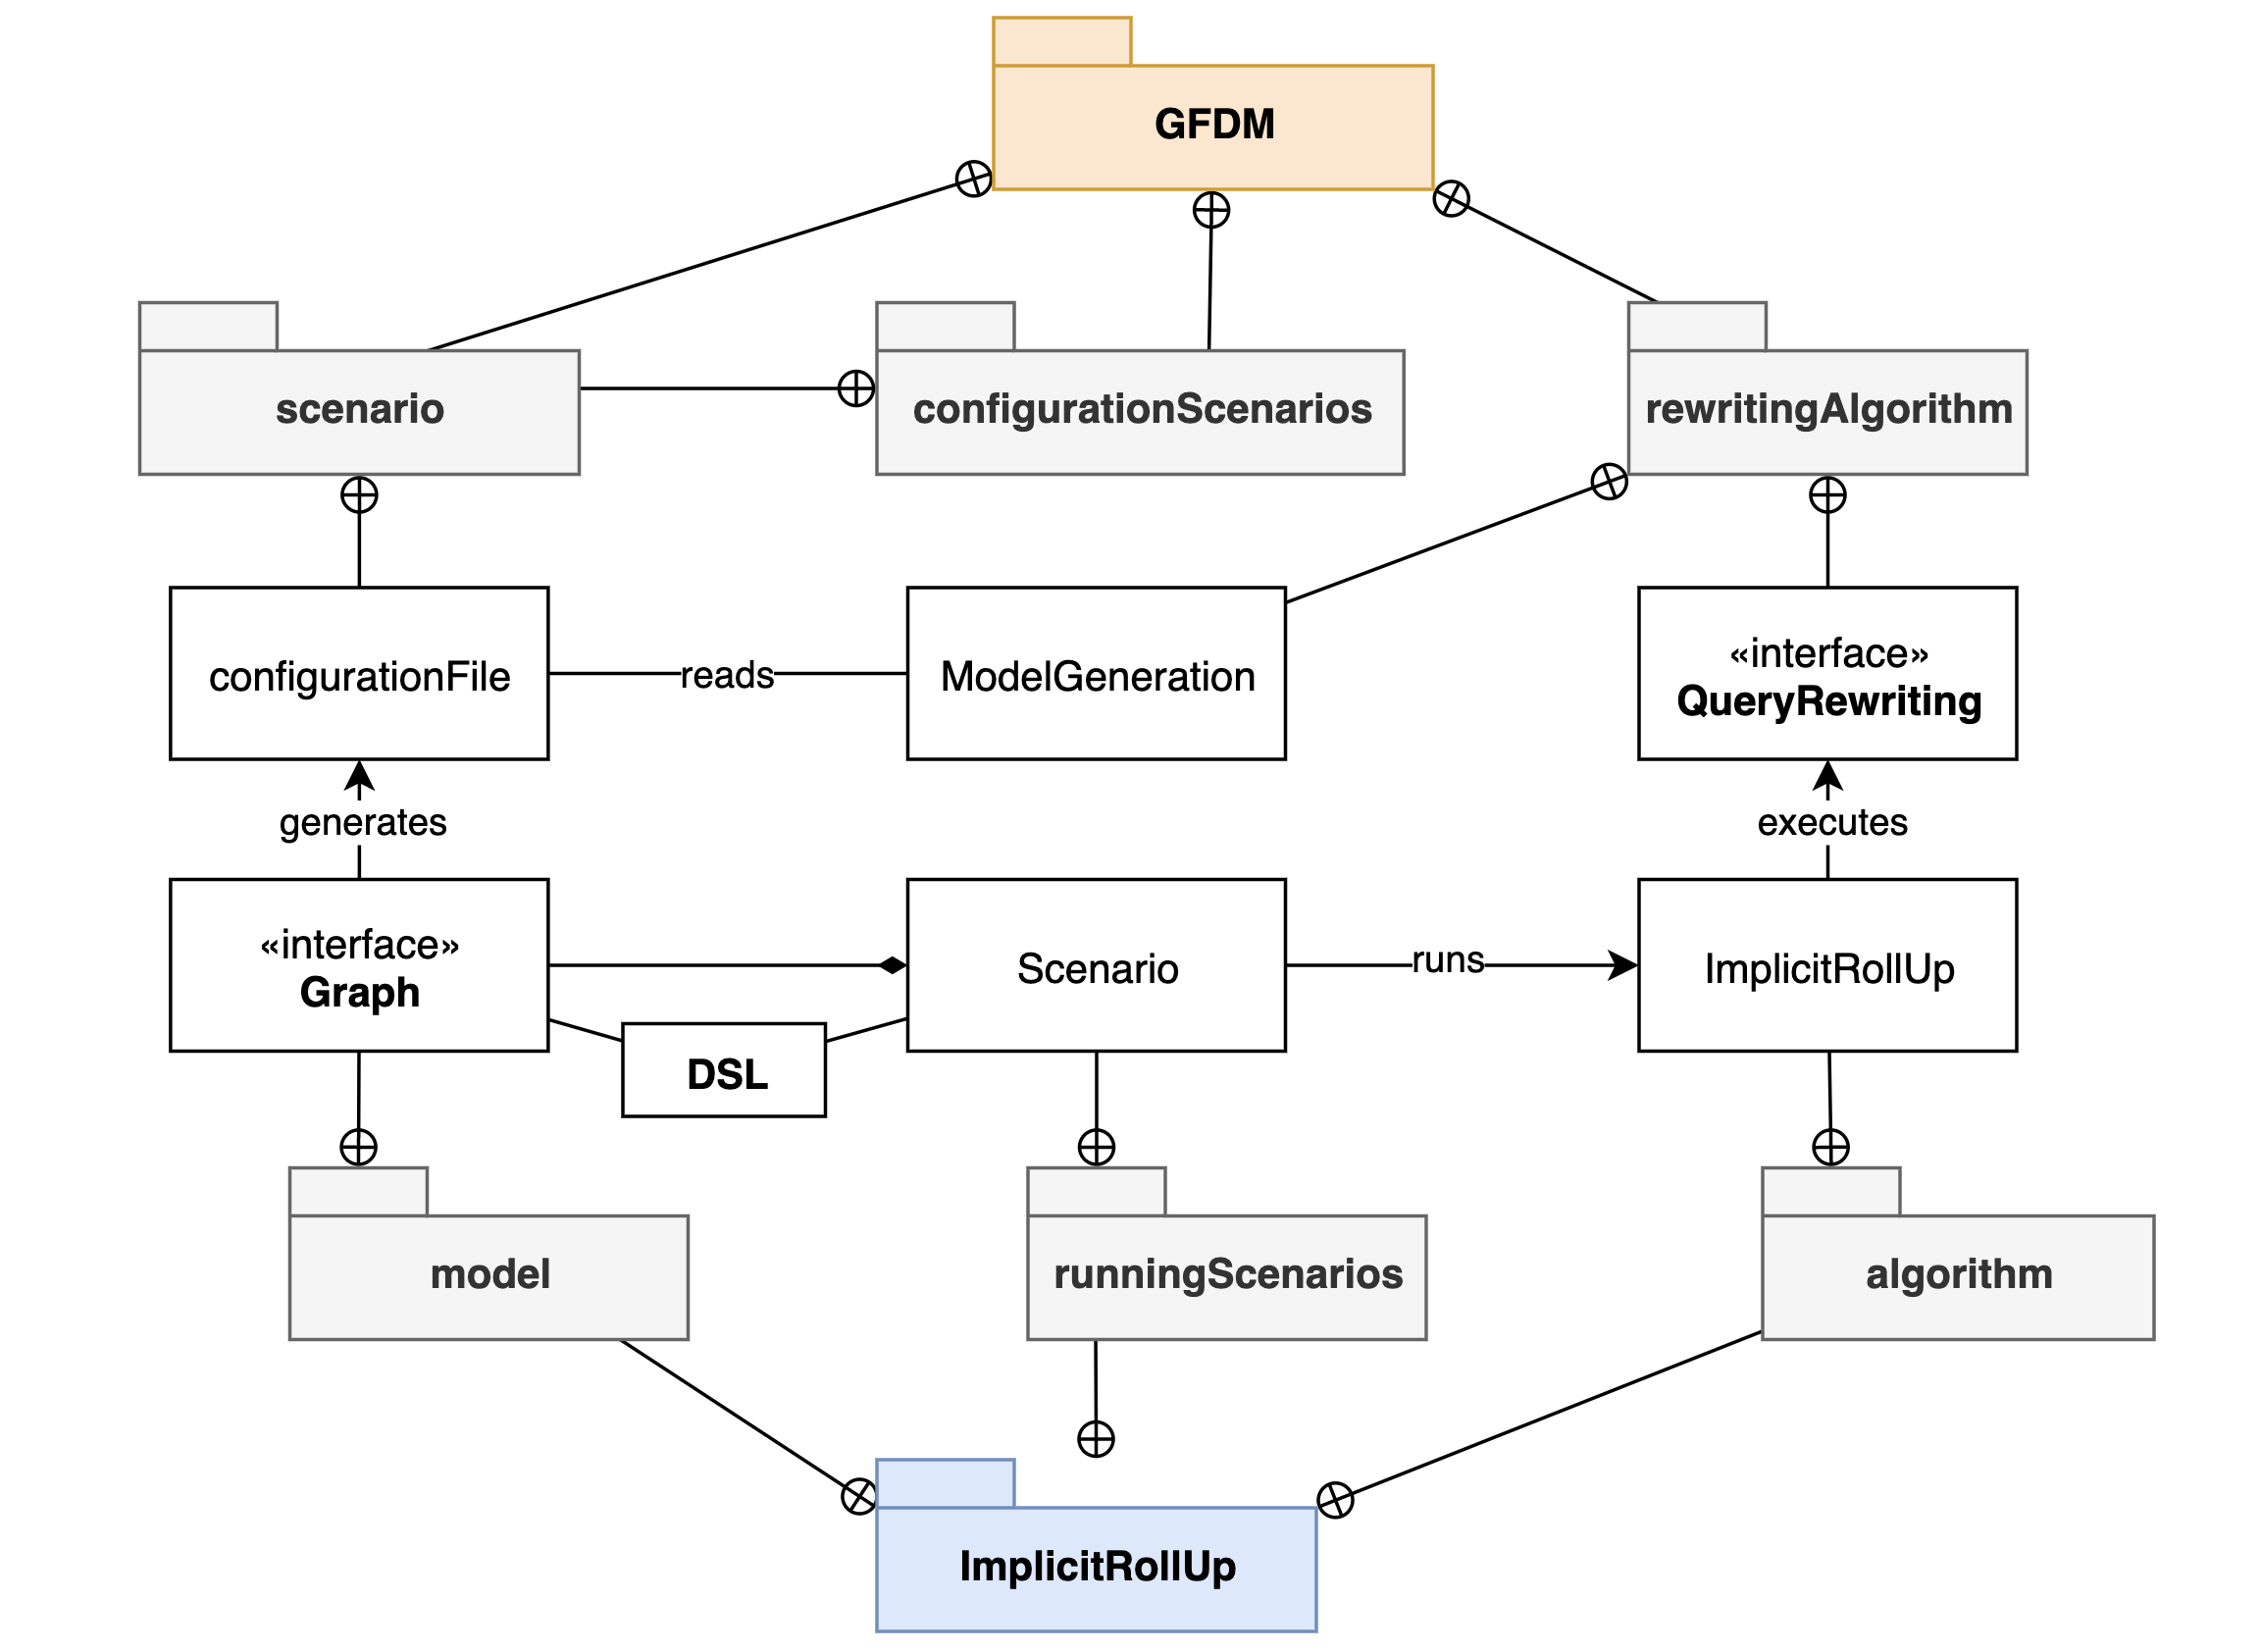
\includegraphics[width=\linewidth]{img/packages.png}}
    \caption{UML package diagram.}
    \label{fig:Package}
\end{figure}
%

\section{Execution flow}
The sequence diagram in figure \ref{fig:Sequence} is describing clearly how the communication between the different modules is performed.
%
The execution flow starts in a \textit{Scenario} where using the DSL or not both the semantic of $\integrationGraph$ and the scenario will be described.
%
The \textit{Utils} module contains the automation flaw that generates all the configuration files (described in section \ref{Functional Requirements}) that \systemName\, needs.
%
Right after the \textit{ImplicitRollUp} module will execute the implicit Roll-Up algorithm that is also described in section \ref{Implicit RollUp}.
%
The implicit Roll-Up algorithm will also need the rewriting algorithm module to execute the query rewriting and producing a relational algebra expression that will be converted in a SQL expression by the module \textit{Sql}.
%
\begin{figure} [ht]
    \fbox{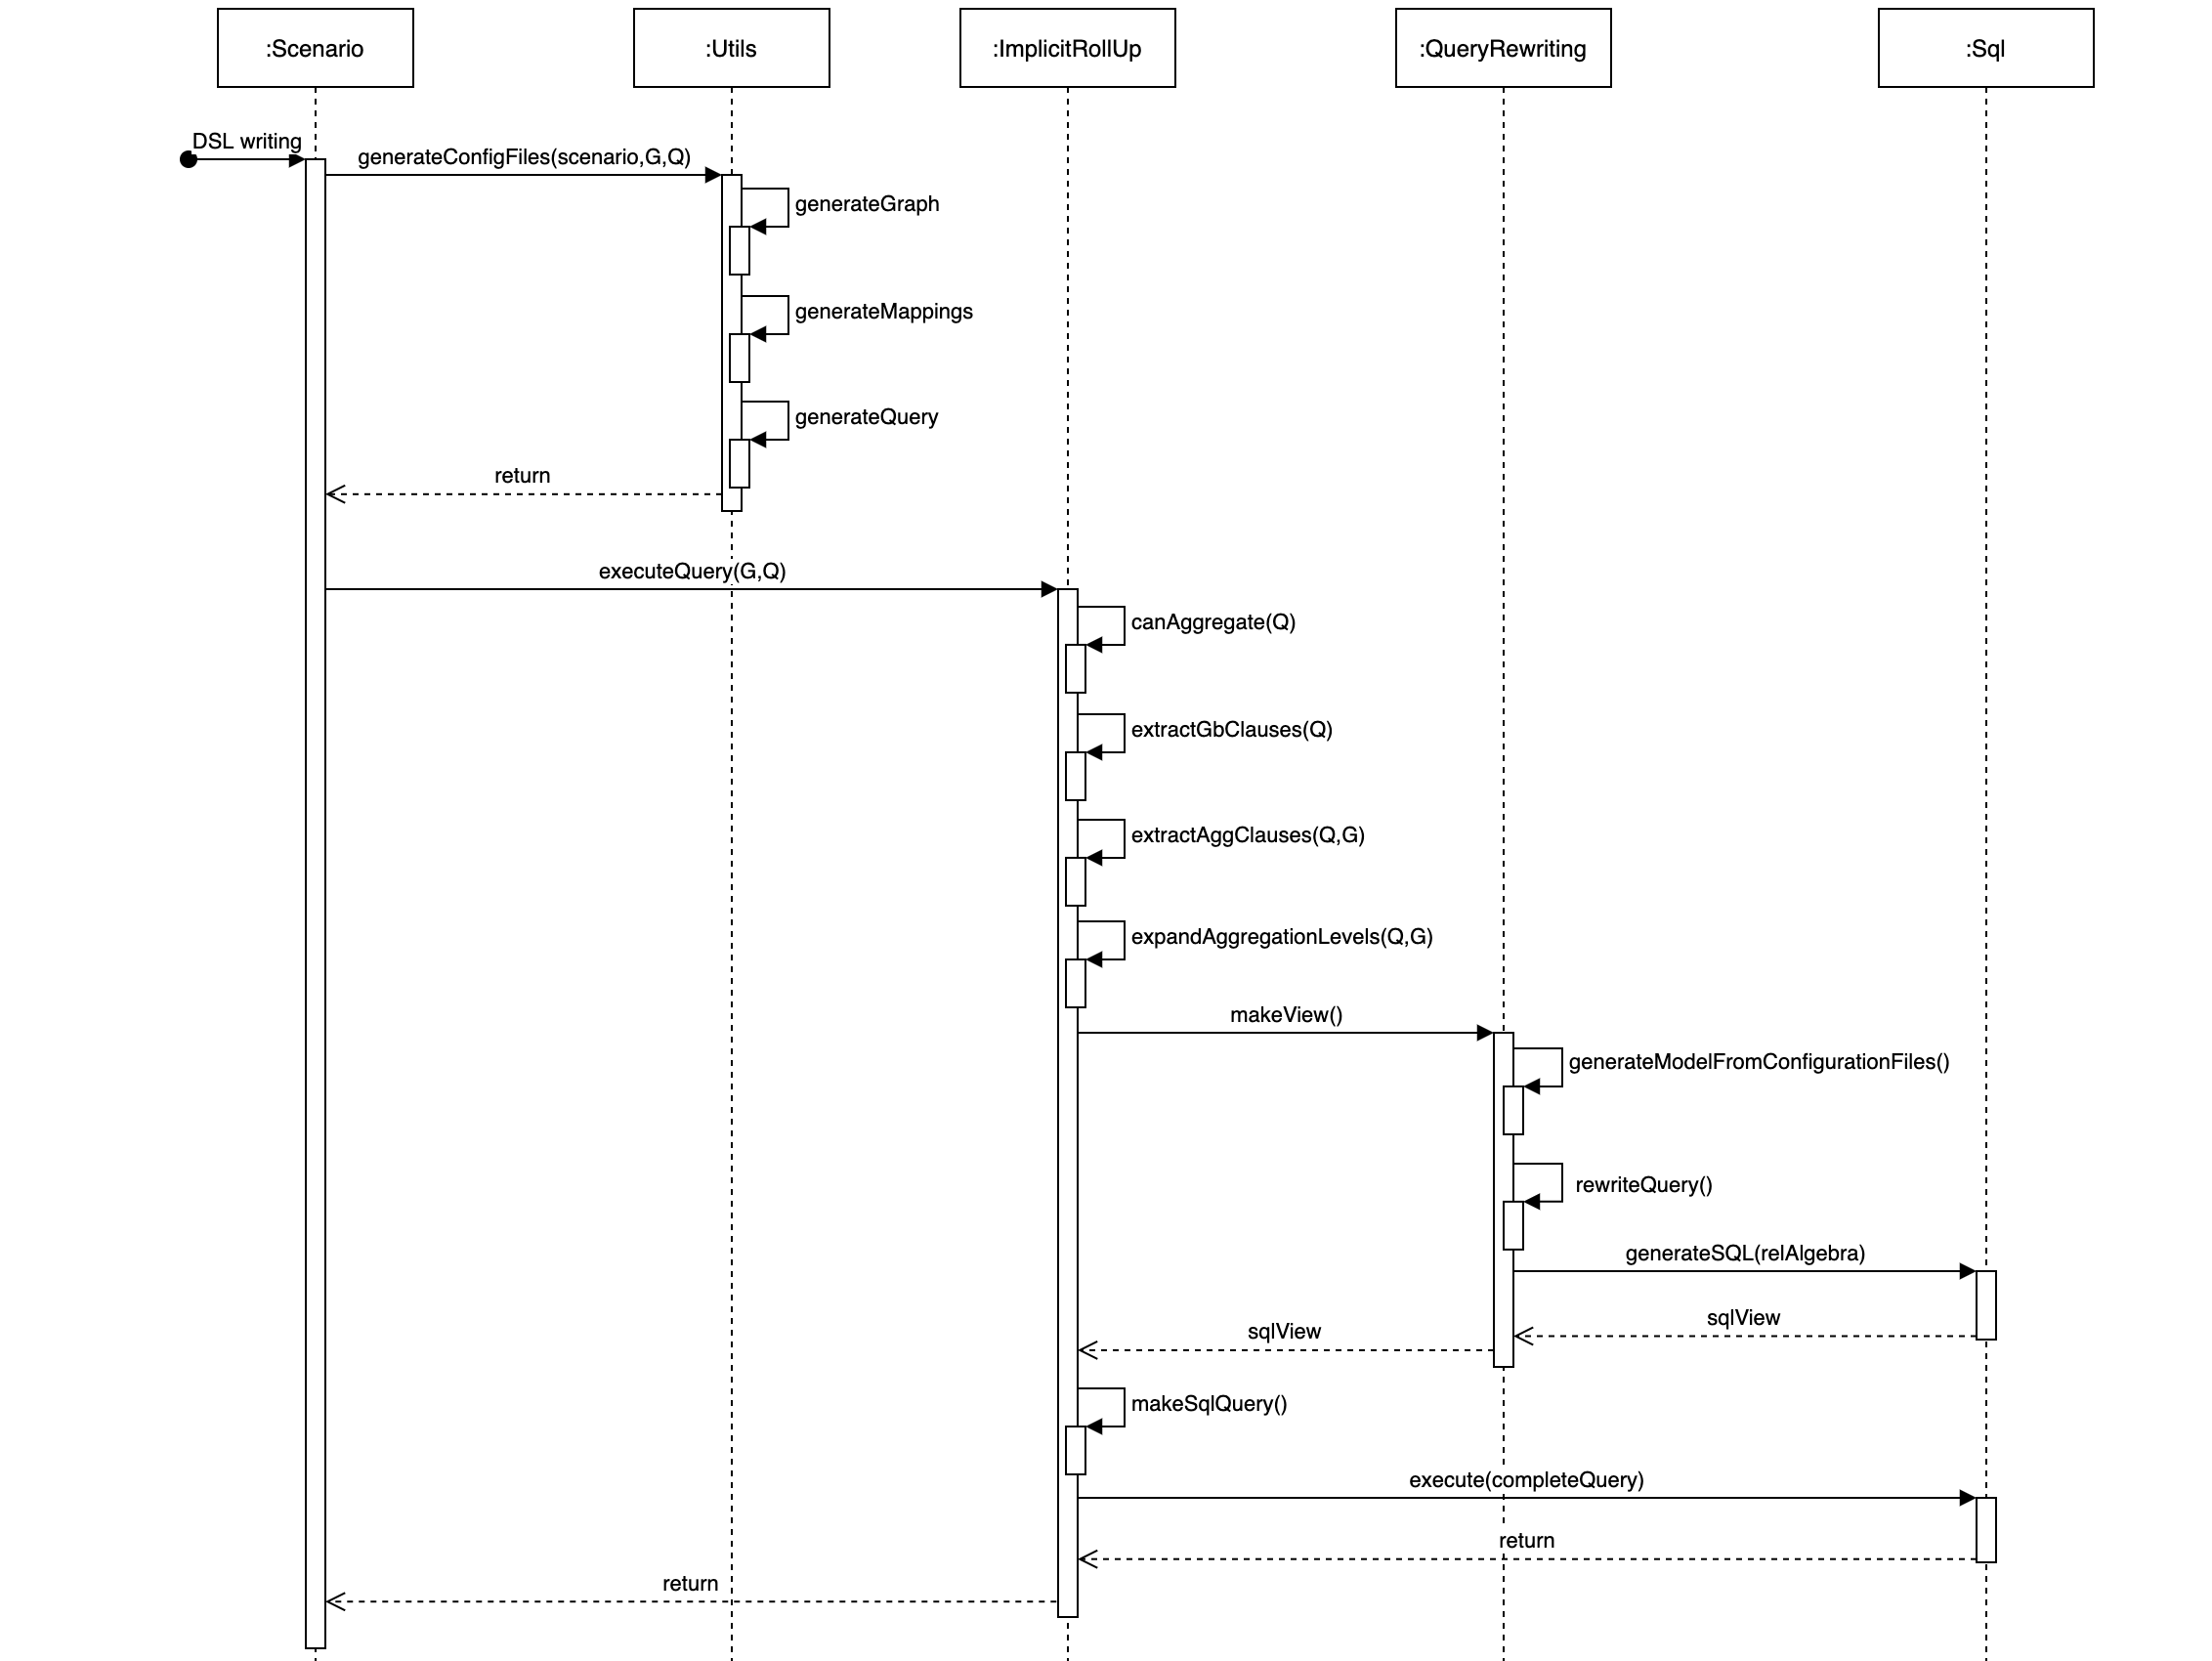
\includegraphics[width=\linewidth]{img/sequence.png}}
    \caption{UML sequence diagram.}
    \label{fig:Sequence}
\end{figure}
%


\section{Domain Specific Language} \label{Domain Specific Language}
In this section will follow some code snippets describing the grammar of the DSL (domain specific language).
%
In particular two kind of DSL have been developed; The first one is related to the generation of the integration graph $\integrationGraph$ and the second is specific to the generation of a configuration scenario.

Let's start with a code snippet that will show how to build $\integrationGraph$.
%
On the top side of the code will be defined all the feature we would like to use.
%
After it will be defined $\integrationGraph$ using the intuitive semantic of the DSL.
%
As we know $\integrationGraph$ is composed both by $\multidimensionalGraph$ and $\sourceGraph$.
%
The first listing starts describing $\multidimensionalGraph$.
%
Since $\globalQuery$ is subsumed by $\multidimensionalGraph$ we have the same syntax for the definition of a query.
%
\begin{lstlisting}[caption={My Caption},style=myScalastyle] 
val REGION = IdFeature("Region")
val COUNTRY = IdFeature("Country")

val NAME = IdFeature("Name")
val CATEGORY = IdFeature("Category")

val REVENUE = Measure("Revenue")

val multidimensionalGraph = 
    Concept("Sales")
      .hasFeature {REVENUE}
      .->("location") { // Concept to concept/level relationship
        Level("Region")
          .hasFeature {REGION}
          .partOf { // Level to level relationship
            Level("Country")
              .hasFeature {COUNTRY}
          }
      }
      .->("product") {
        Level("Name")
          .hasFeature {NAME}
          .partOf {
            Level("Category")
              .hasFeature {CATEGORY}
          }
      }
\end{lstlisting}
%
The second listing describes the DSL for the generation of $\sourceGraph$.
%
It will be possible to define both wrappers and attributes and to describe the $\sameAs$ relationship with $\feature$.
%
\begin{lstlisting}[caption={My Caption},style=myScalastyle] 
val w1 = 
    Wrapper("W1")
      .hasAttribute {
        Attribute("country") sameAs COUNTRY
      }
      .hasAttribute {
        Attribute("region") sameAs REGION
      }
      .hasAttribute {
        Attribute("revenue") sameAs REVENUE
      }
\end{lstlisting}
%
Finally the last DSL proposed will help dealing with the generation of a scenario an also the run of the scenario itself.
%
As we know a scenario is composed by the scenario name, a target graph, that can be both $\targetGraph$ or $\multidimensionalGraph$, all the wrappers, all the aggregation functions and finally the query.
%
\begin{lstlisting}[caption={My Caption},style=myScalastyle]
class ScenarioName extends Scenario {
  scenario {
    "ScenarioName"
  }

  targetGraph{
    // The target graph
  }

  wrapper {
    // One wrapper, if there are more than one repeat this block
  }
  
  query {
    // The query
  }
  
  aggregation {
    // One aggregation function, if there are more than one repeat this block
  }

}
\end{lstlisting}
%
Finally once crated the scenario, it will be possible to run it and flag if running implicit Roll-Up or not.
%
\begin{lstlisting}[caption={My Caption},style=myScalastyle]
object ScenarioName extends App {
  new ScenarioName().run(executeImplicitRollUp = true)
}
\end{lstlisting}


\chapter{Experimentation}

\section{Automatic test}

\section{Validation test}
Description of the experimental datasets and experiments conducted. Report results and interpret them.

The only factor that matters for performances is the size of the graph.

\chapter{Conclusions and future works}
% Summing up.
%Open repository for dimensional lookup table.



\chapter{Problems, \textit{to drop}}

\begin{itemize}
    \item Aggregation functions are separate form $\multidimensionalGraph$ in my implementation, I cheat passing to the implicit Roll-Up algorithm a set of aggregation function, that are actually graphs.
    %
    \item How to chose the right id to expand for a Level if there are multiple… I may need AggregationId but also not (I can cut form the rewriting actually)
    \item partOf relationship, Dimensions and Facts are very relaxed in my work because are not necessary for the algorithm, but they may be very useful for understanding the model and for visualisation purpose and managing for future works.
    \item disjointedness of data (assume disjointedness) and compatibility (assume compatibility)
    \item Data set showcases (assume not to have all the hierarchy filled in one variable), otherwise we may need to enrich the model
    \item The algorithm is faked a bit in section \ref{Implicit RollUp} to make it more understandable (eg hide that \systemName works with configuration files)
    \item include wrapper name in the result is not implemented
\end{itemize}

\begin{thebibliography}{9}
\bibitem{TKDE} 
Nadal, S., Abello, A., Romero, O., Vansummeren, S., and Vassiliadis, P. (2021). Graph-driven Federated Data Management. IEEE Transactions On Knowledge And Data Engineering, 1-1. doi: 10.1109/tkde.2021.3077044


\end{thebibliography}

\end{document}

